\documentclass[11pt, a4paper]{article}

\usepackage{amsfonts}
\usepackage{amssymb}
\usepackage{amsmath}
\usepackage{epsfig}
\usepackage{graphicx}
\usepackage{tabularx}
\usepackage{parskip}
\usepackage[margin=2.54cm]{geometry}
\usepackage[colorlinks=true]{hyperref}
\usepackage[sort]{natbib}

%%%%%%%%%%%%%%%%%%%%%%%%%%%%%%%%%%%%%%%%%%%%%%%%%%%%%%%%%%%%%%%%%%%%%%%%%%%%%%%%%
%%%%%%%%%%%%%%%%%%%%%%%%%%%%%%%%%%%%%%%%%%%%%%%%%%%%%%%%%%%%%%%%%%%%%%%%%%%%%%%%%
\title{Tag growth}

\author{D'Arcy N. Webber, Jim Thorson}

\date{\today}

\begin{document}
\maketitle

%%%%%%%%%%%%%%%%%%%%%%%%%%%%%%%%%%%%%%%%%%%%%%%%%%%%%%%%%%%%%%%%%%%%%%%%%%%%%%%%%
%%%%%%%%%%%%%%%%%%%%%%%%%%%%%%%%%%%%%%%%%%%%%%%%%%%%%%%%%%%%%%%%%%%%%%%%%%%%%%%%%
%%%%%%%%%%%%%%%%%%%%%%%%%%%%%%%%%%%%%%%%%%%%%%%%%%%%%%%%%%%%%%%%%%%%%%%%%%%%%%%%%
\section{Introduction}
%%%%%%%%%%%%%%%%%%%%%%%%%%%%%%%%%%%%%%%%%%%%%%%%%%%%%%%%%%%%%%%%%%%%%%%%%%%%%%%%%
%%%%%%%%%%%%%%%%%%%%%%%%%%%%%%%%%%%%%%%%%%%%%%%%%%%%%%%%%%%%%%%%%%%%%%%%%%%%%%%%%
%%%%%%%%%%%%%%%%%%%%%%%%%%%%%%%%%%%%%%%%%%%%%%%%%%%%%%%%%%%%%%%%%%%%%%%%%%%%%%%%%
\textit{Dissostichus mawsoni}

Key words: Antarctic toothfish, Ross Sea


\begin{equation}
  \frac{dL}{dt} = a - k L,
\end{equation}

\begin{equation}
  a = \gamma k^\psi,
\end{equation}
When $\psi = 0$ this model become the classic von Bertallanffy.

\begin{align}
  \frac{dL}{dt} &= \gamma k^\psi - k L,\\
  &= \gamma - k L \quad \text{if} \quad \psi = 0,
\end{align}

\begin{align}
  L_\infty &= \frac{\gamma k^\psi}{k},\\
  &= \frac{\gamma}{k} \quad \text{if} \quad \psi = 0, 
\end{align}

\begin{align}
  \gamma &= \frac{k L_\infty}{k^\psi},\\
  &= k L_\infty \quad \text{if} \quad \psi = 0, 
\end{align}


\begin{equation}
  L_0 = L_\infty \left( 1 - e^{k t_0} \right),
\end{equation}
$L_0$ is the length at time 0.

\begin{align}
  c_v &= \frac{\sigma}{\mu},\\
  \sigma &= c_v \mu,\\
  \varepsilon &\sim \mathcal{N} \left( 0, \sigma^2_o L_t \right),
\end{align}


\begin{table}[!htbp]
  \begin{quote}
    \caption{\label{tab:Dunn} .} \small{
      \begin{center}
        \begin{tabular}{lrr}
          \hline
          Parameter      & Female & Male\\
          \hline
          $t_0$ (y) & 0.021 & -0.256\\
          $k$ ($\text{y}^{-1}$) & 0.090 & 0.093\\
          $L_\infty$ (cm) & 180.20 & 169.07\\
          $c_v$ & 0.102 & 0.012\\
          \hline
        \end{tabular}
      \end{center}
    }
  \end{quote}
\end{table}

\begin{equation}
  L_t = L_\infty \left( 1 - e^{-k (t - t_0)} \right),
\end{equation}


%%%%%%%%%%%%%%%%%%%%%%%%%%%%%%%%%%%%%%%%%%%%%%%%%%%%%%%%%%%%%%%%%%%%%%%%%%%%%%%%%
%%%%%%%%%%%%%%%%%%%%%%%%%%%%%%%%%%%%%%%%%%%%%%%%%%%%%%%%%%%%%%%%%%%%%%%%%%%%%%%%%
%%%%%%%%%%%%%%%%%%%%%%%%%%%%%%%%%%%%%%%%%%%%%%%%%%%%%%%%%%%%%%%%%%%%%%%%%%%%%%%%%
\section{Simulation}
%%%%%%%%%%%%%%%%%%%%%%%%%%%%%%%%%%%%%%%%%%%%%%%%%%%%%%%%%%%%%%%%%%%%%%%%%%%%%%%%%
%%%%%%%%%%%%%%%%%%%%%%%%%%%%%%%%%%%%%%%%%%%%%%%%%%%%%%%%%%%%%%%%%%%%%%%%%%%%%%%%%
%%%%%%%%%%%%%%%%%%%%%%%%%%%%%%%%%%%%%%%%%%%%%%%%%%%%%%%%%%%%%%%%%%%%%%%%%%%%%%%%%
Simulated 315 individuals, the same number as in the actual toothfish data
set. The next step was to simulate sex, Age1, Age2 and time at liberty. What I
did in the current simulation run was:
\begin{itemize}
\item Sampled sex from the observed sexes of individuals (with replacement).
\item Sampled Age1, Age2 and time at liberty independently (with replacement)
  from those observed. Randomly selected one of these variables and calculated
  this values given the other two.
\item Rounded Age1, Age2 and time at liberty off to the nearest integer.
\end{itemize}
This is a bit of a hack I know, but the alternative did not yeild realistic
looking Age1, Age2, liberty samples.



\newpage\clearpage
%%%%%%%%%%%%%%%%%%%%%%%%%%%%%%%%%%%%%%%%%%%%%%%%%%%%%%%%%%%%%%%%%%%%%%%%%%%%%%%%%
%%%%%%%%%%%%%%%%%%%%%%%%%%%%%%%%%%%%%%%%%%%%%%%%%%%%%%%%%%%%%%%%%%%%%%%%%%%%%%%%%
\subsection{Fits to simulated data}
%%%%%%%%%%%%%%%%%%%%%%%%%%%%%%%%%%%%%%%%%%%%%%%%%%%%%%%%%%%%%%%%%%%%%%%%%%%%%%%%%
%%%%%%%%%%%%%%%%%%%%%%%%%%%%%%%%%%%%%%%%%%%%%%%%%%%%%%%%%%%%%%%%%%%%%%%%%%%%%%%%%

%%%%%%%%%%%%%%%%%%%%%%%%%%%%%%%%%%%%%%%%%%%%%%%%%%%%%%%%%%%%%%%%%%%%%%%%%%%%%%%%%
\subsubsection{sims1}
%%%%%%%%%%%%%%%%%%%%%%%%%%%%%%%%%%%%%%%%%%%%%%%%%%%%%%%%%%%%%%%%%%%%%%%%%%%%%%%%%
This was our first attempt at estimating simulated data.  $L_0$ was simulated
as 43 and 50 for females and males respectively (Table~\ref{tab:sims1}).

$L_0$ was estimated without a prior penalty.  $b$ was treated as a random
effect.

80 of 100 fits were pdHess.  Looking at the histograms below there seems to be
two states that the model estimates are jumping between.  Looking at the trace
plots, when $\sigma_o$ is estimated high then the remaining parameters are
poorly estimated (Figure~\ref{fig:sims1}).
\begin{table}[!htbp]
  \begin{quote}
    \caption{\label{tab:sims1} .} \small{
      \begin{center}
        \begin{tabular}{lrr}
          \hline
          Parameter      & Female & Male\\
          \hline
          $L_0$          & 43   & 50\\
          $\overline{b}$ & 0.00100 & 0.00106\\
          $\sigma_b$     & 0.21 & 0.19\\
          $\gamma$       & 0.19   & 0.19\\
          $\psi$         & 2e-10 & 2e-10\\
          $\sigma_o$     & 0.083 & 0.083\\
          $\sigma_z$     & 0.0   & 0.0\\
          $\sigma_y$     & 0.0   & 0.0\\
          \hline
        \end{tabular}
      \end{center}
    }
  \end{quote}
\end{table}

\begin{figure}[!htbp]
  \centering
  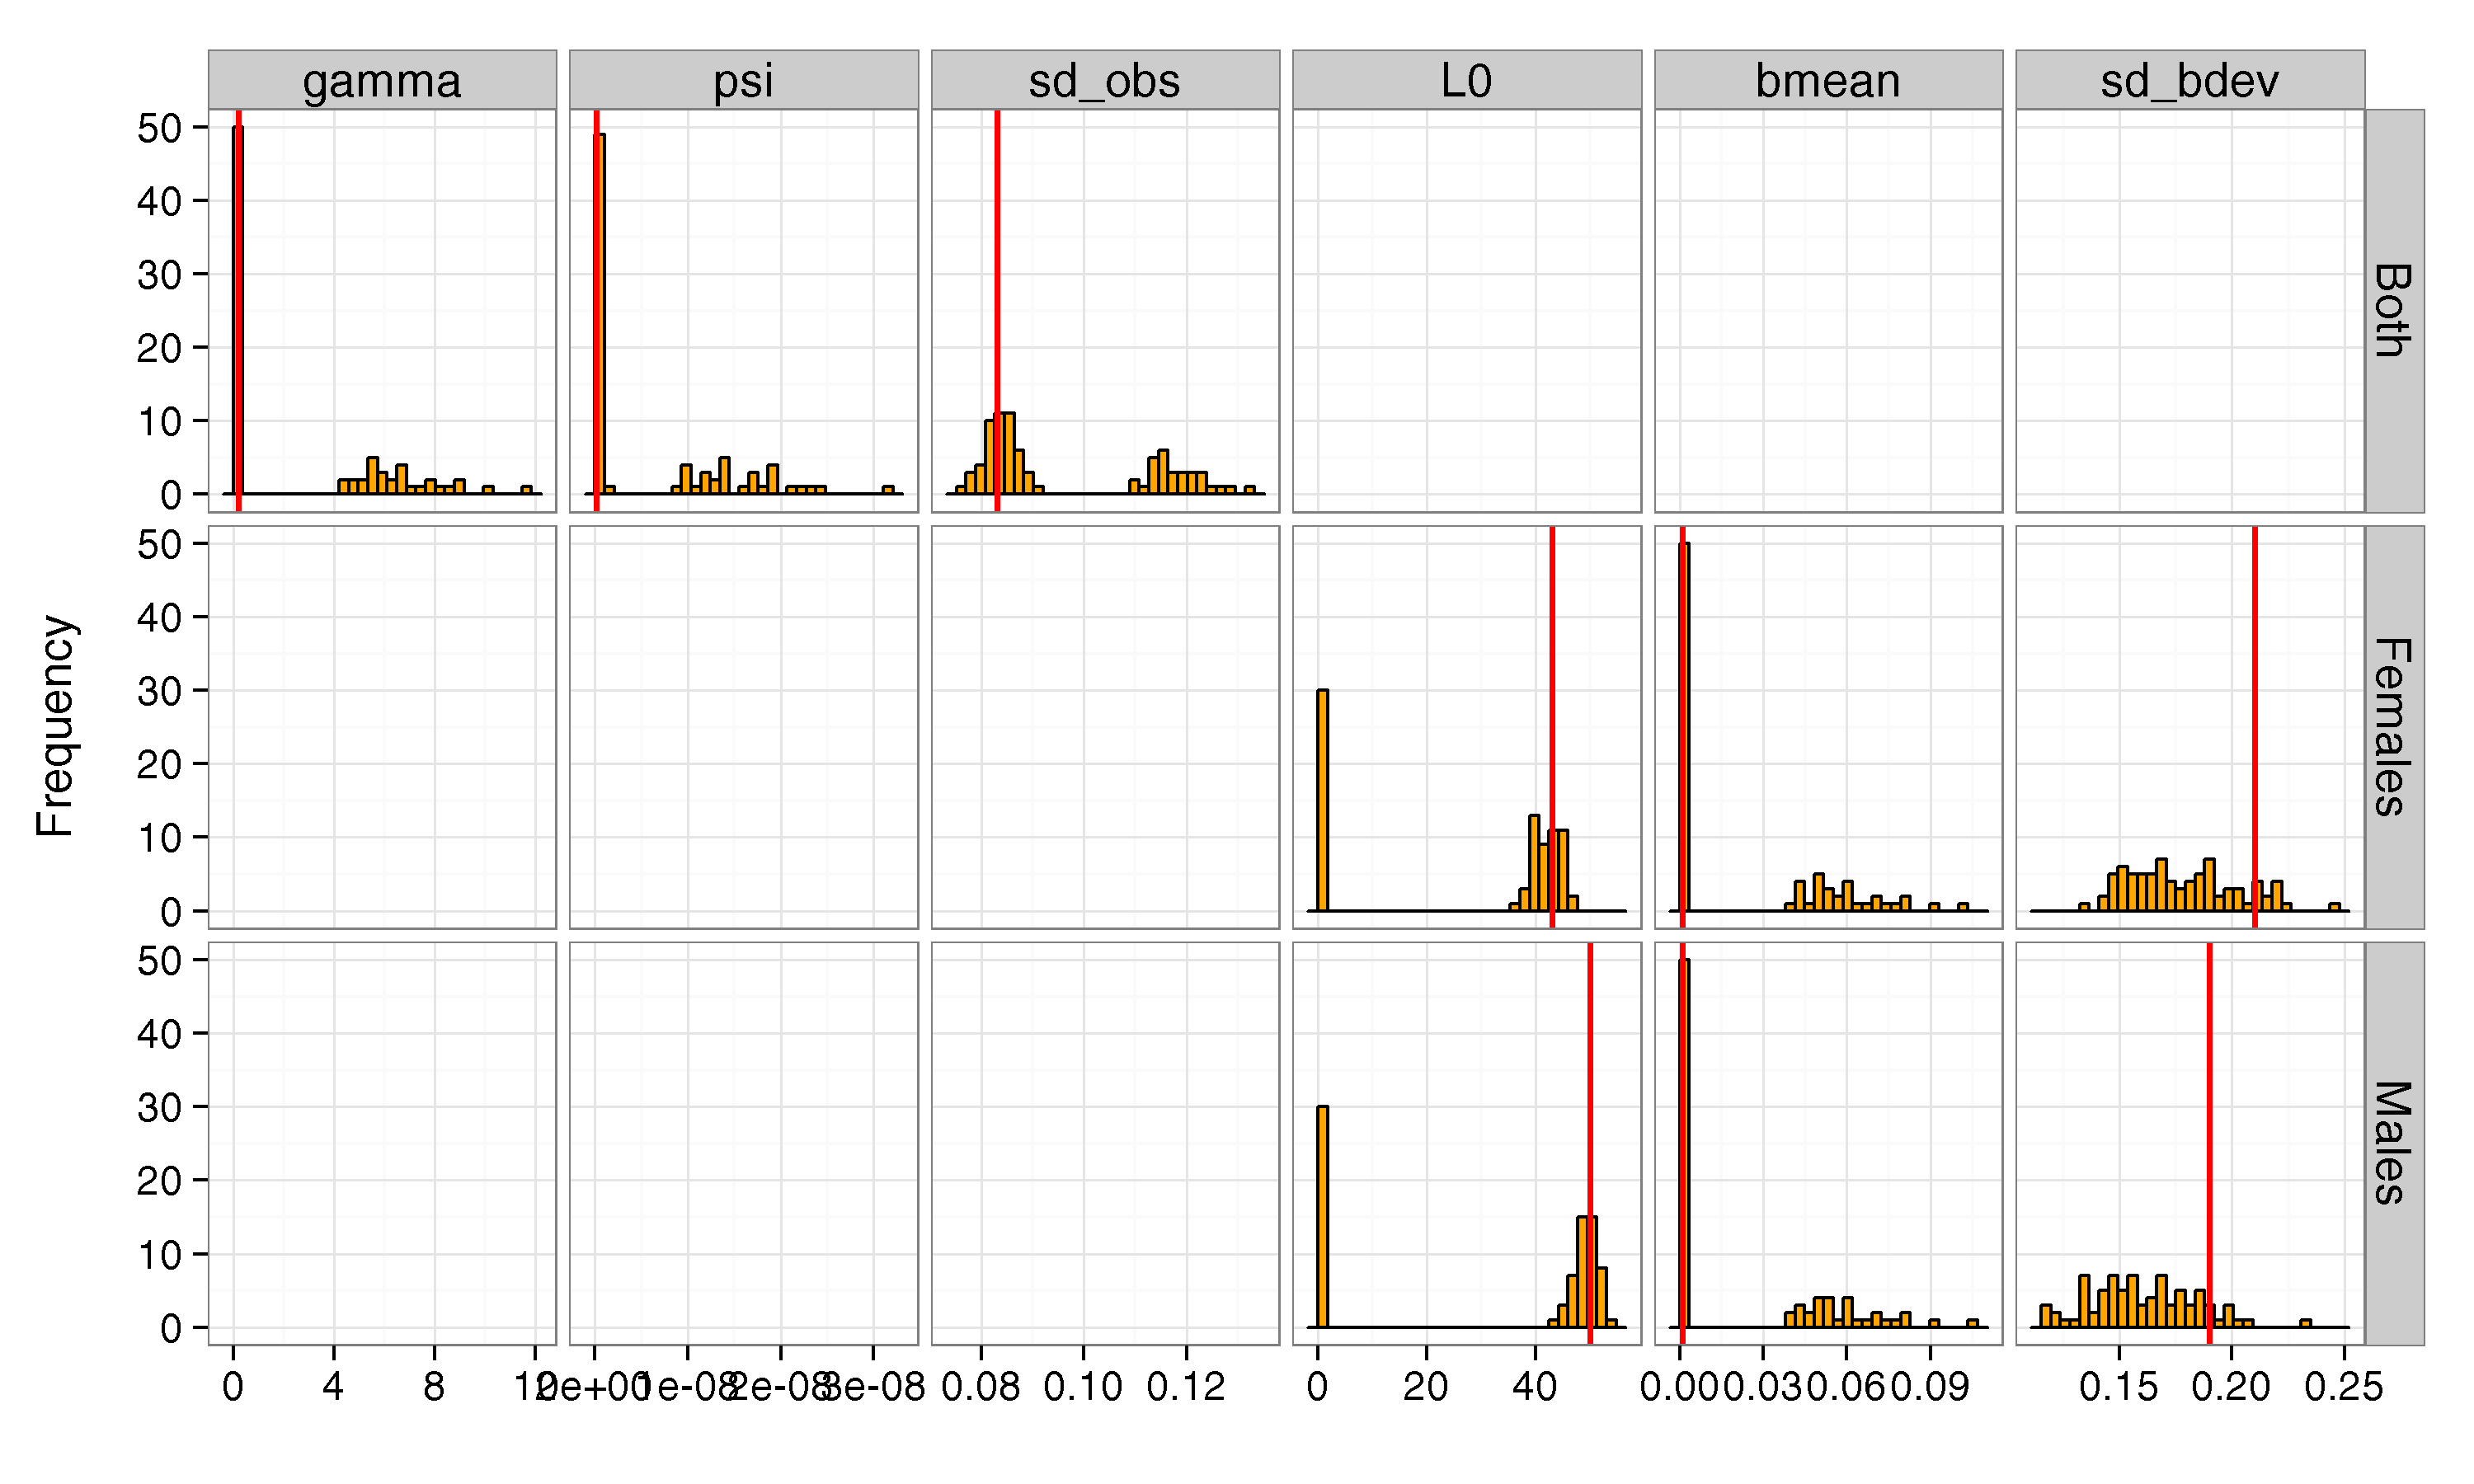
\includegraphics[width=\linewidth]{../simulation/sims1/results/SimPars.png}
  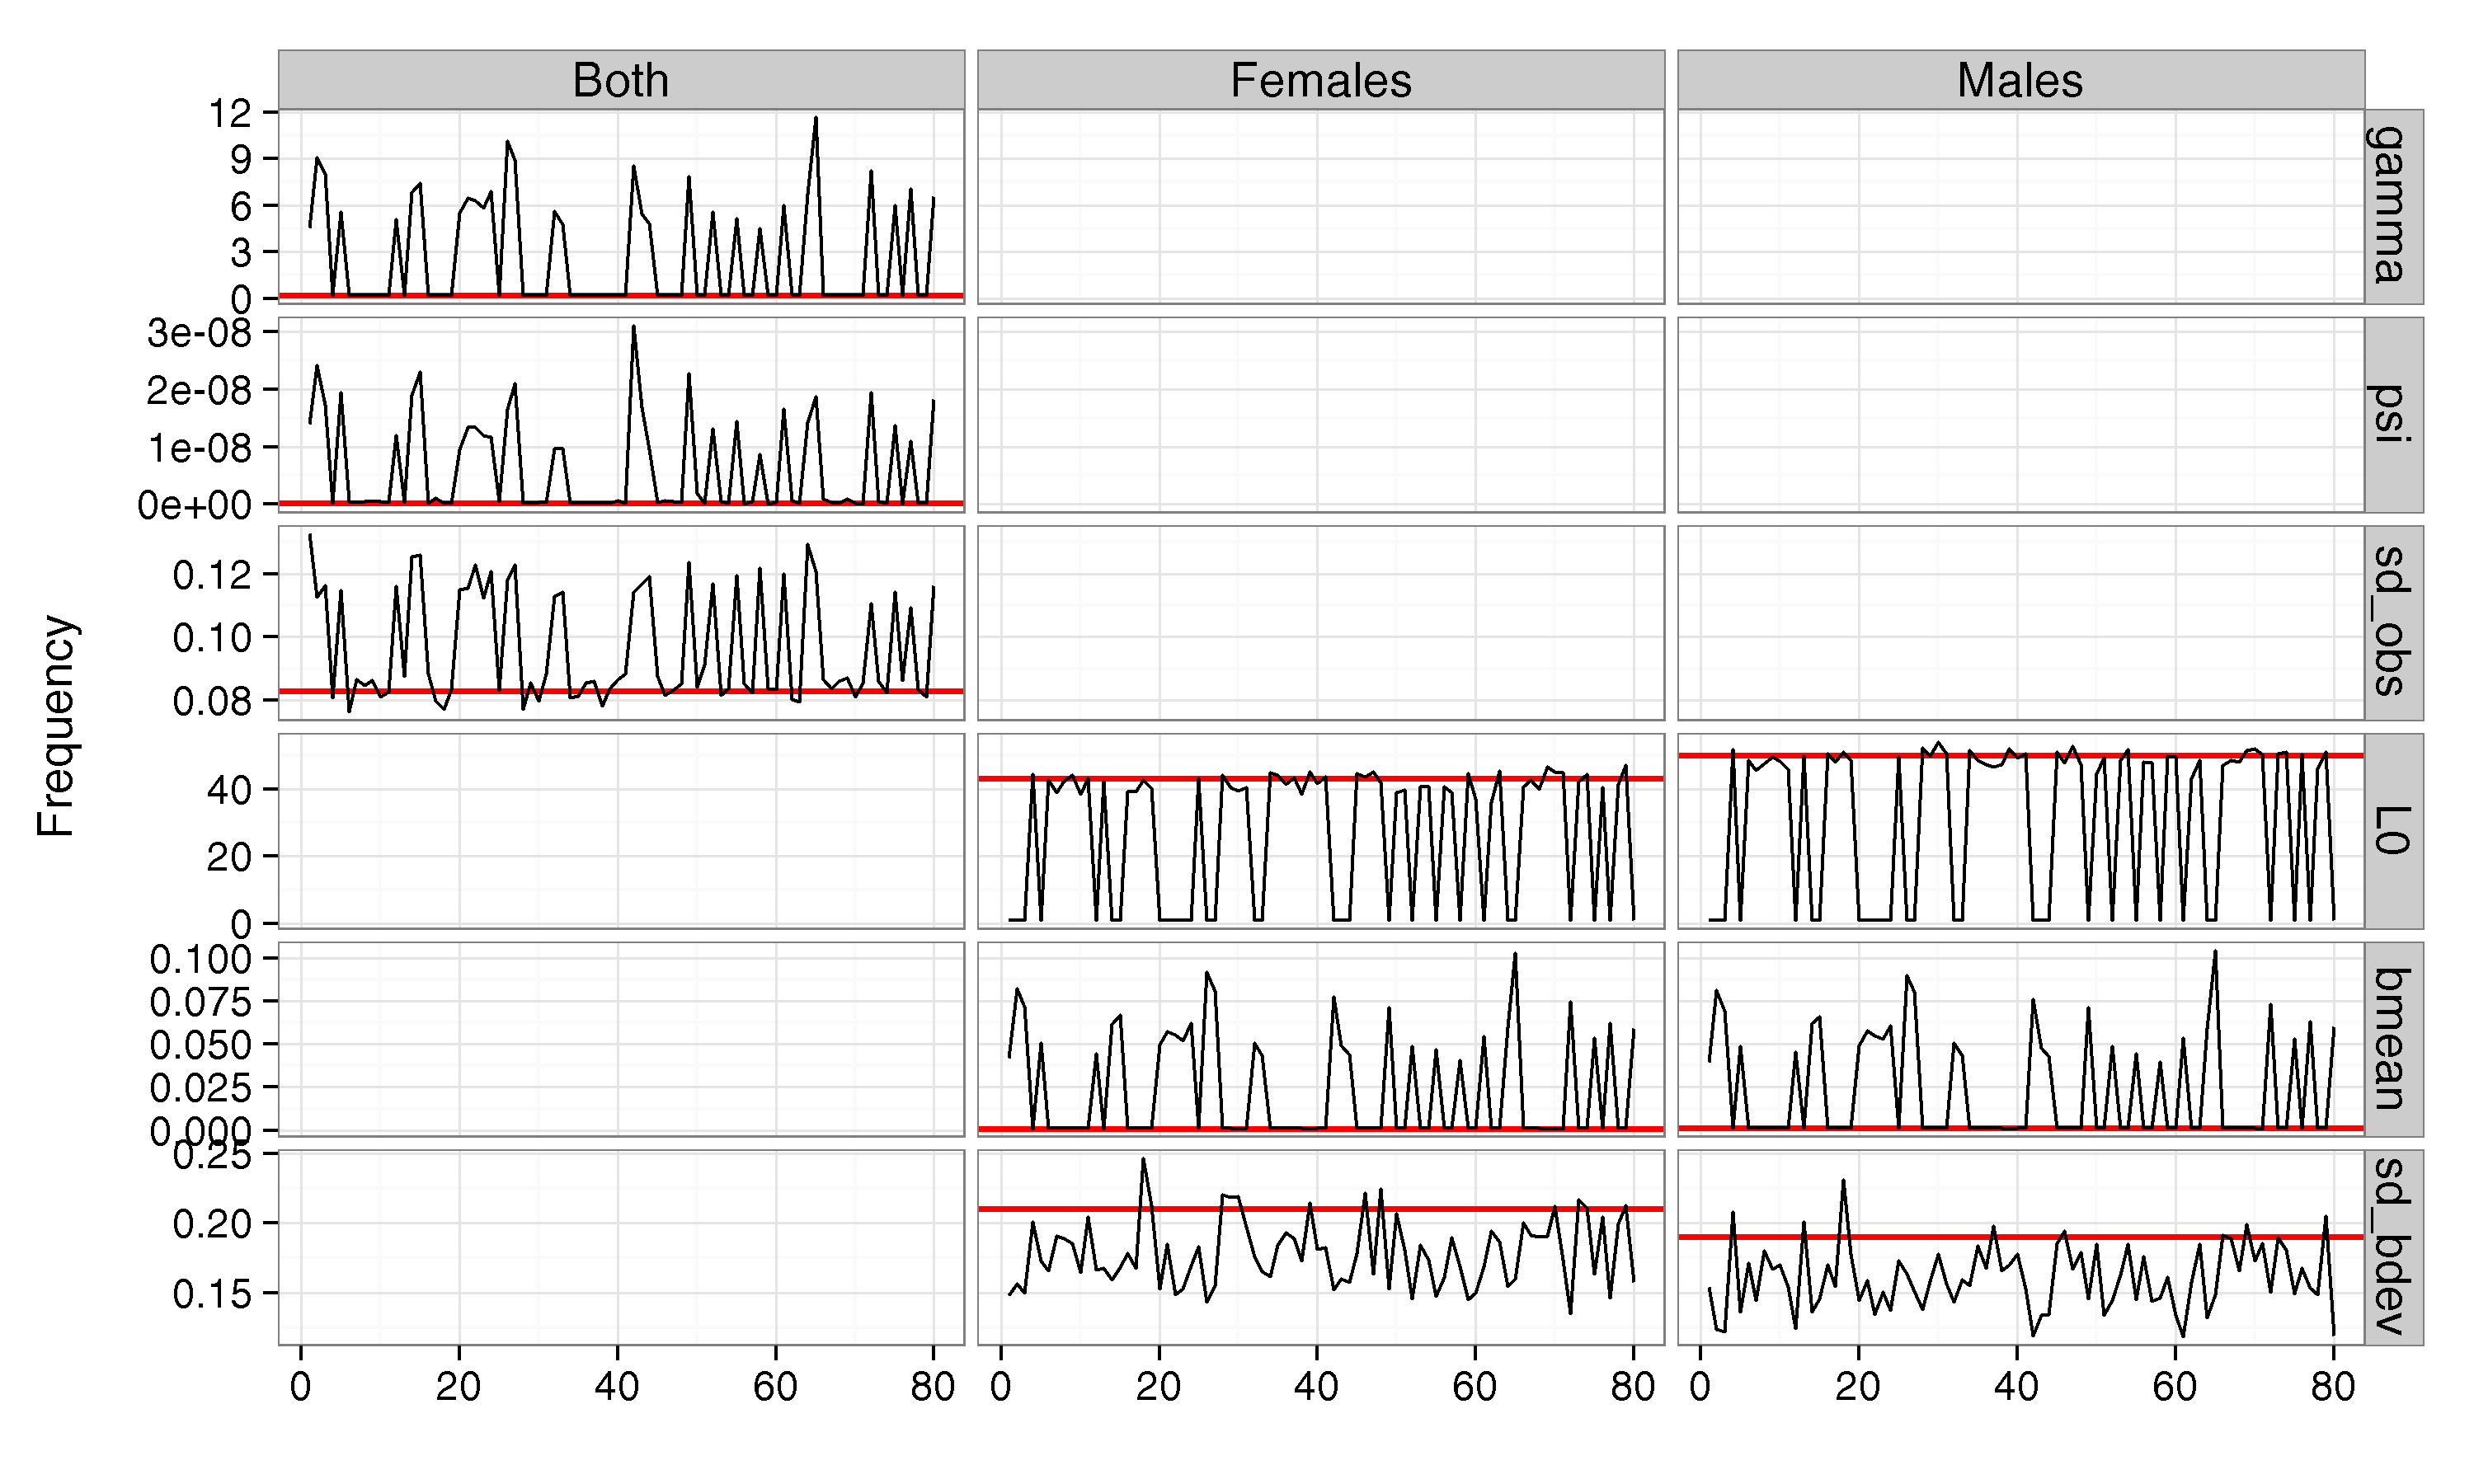
\includegraphics[width=\linewidth]{../simulation/sims1/results/TracePars.png}
  \begin{quote}
    \caption{pdH fits plotted only (80 of 100 fits were pdH)..}
    \label{fig:sims1}
  \end{quote}
\end{figure}


\newpage\clearpage
%%%%%%%%%%%%%%%%%%%%%%%%%%%%%%%%%%%%%%%%%%%%%%%%%%%%%%%%%%%%%%%%%%%%%%%%%%%%%%%%%
\subsubsection{sims2}
%%%%%%%%%%%%%%%%%%%%%%%%%%%%%%%%%%%%%%%%%%%%%%%%%%%%%%%%%%%%%%%%%%%%%%%%%%%%%%%%%
The simulation was run with $L_0$ values much closer to 0
(Table~\ref{tab:sims2}).

We placed a prior penalty on $L_0$ (a normal centered about 0).  Again, $b$ was
treated as a random effect.

57 of 100 fits were pdHess.  Doing a poor job of recovering $L_0$ for males.
Two states that seem to be linked to $\sigma_o$ again.  Not getting $\psi$ at
all (Figure~\ref{fig:sims2}).
\begin{table}[!htbp]
  \begin{quote}
    \caption{\label{tab:sims2} .} \small{
      \begin{center}
        \begin{tabular}{lrr}
          \hline
          Parameter      & Female & Male\\
          \hline
          $L_0$          & 0.0   & 6.9\\
          $\overline{b}$ & 0.003 & 0.003\\
          $\sigma_b$     & 0.106 & 0.112\\
          $\gamma$       & 0.4   & 0.4\\
          $\psi$         & 0.001 & 0.001\\
          $\sigma_o$     & 0.099 & 0.099\\
          $\sigma_z$     & 0.0   & 0.0\\
          $\sigma_y$     & 0.0   & 0.0\\
          \hline
        \end{tabular}
      \end{center}
    }
  \end{quote}
\end{table}

\begin{figure}[!htbp]
  \centering
  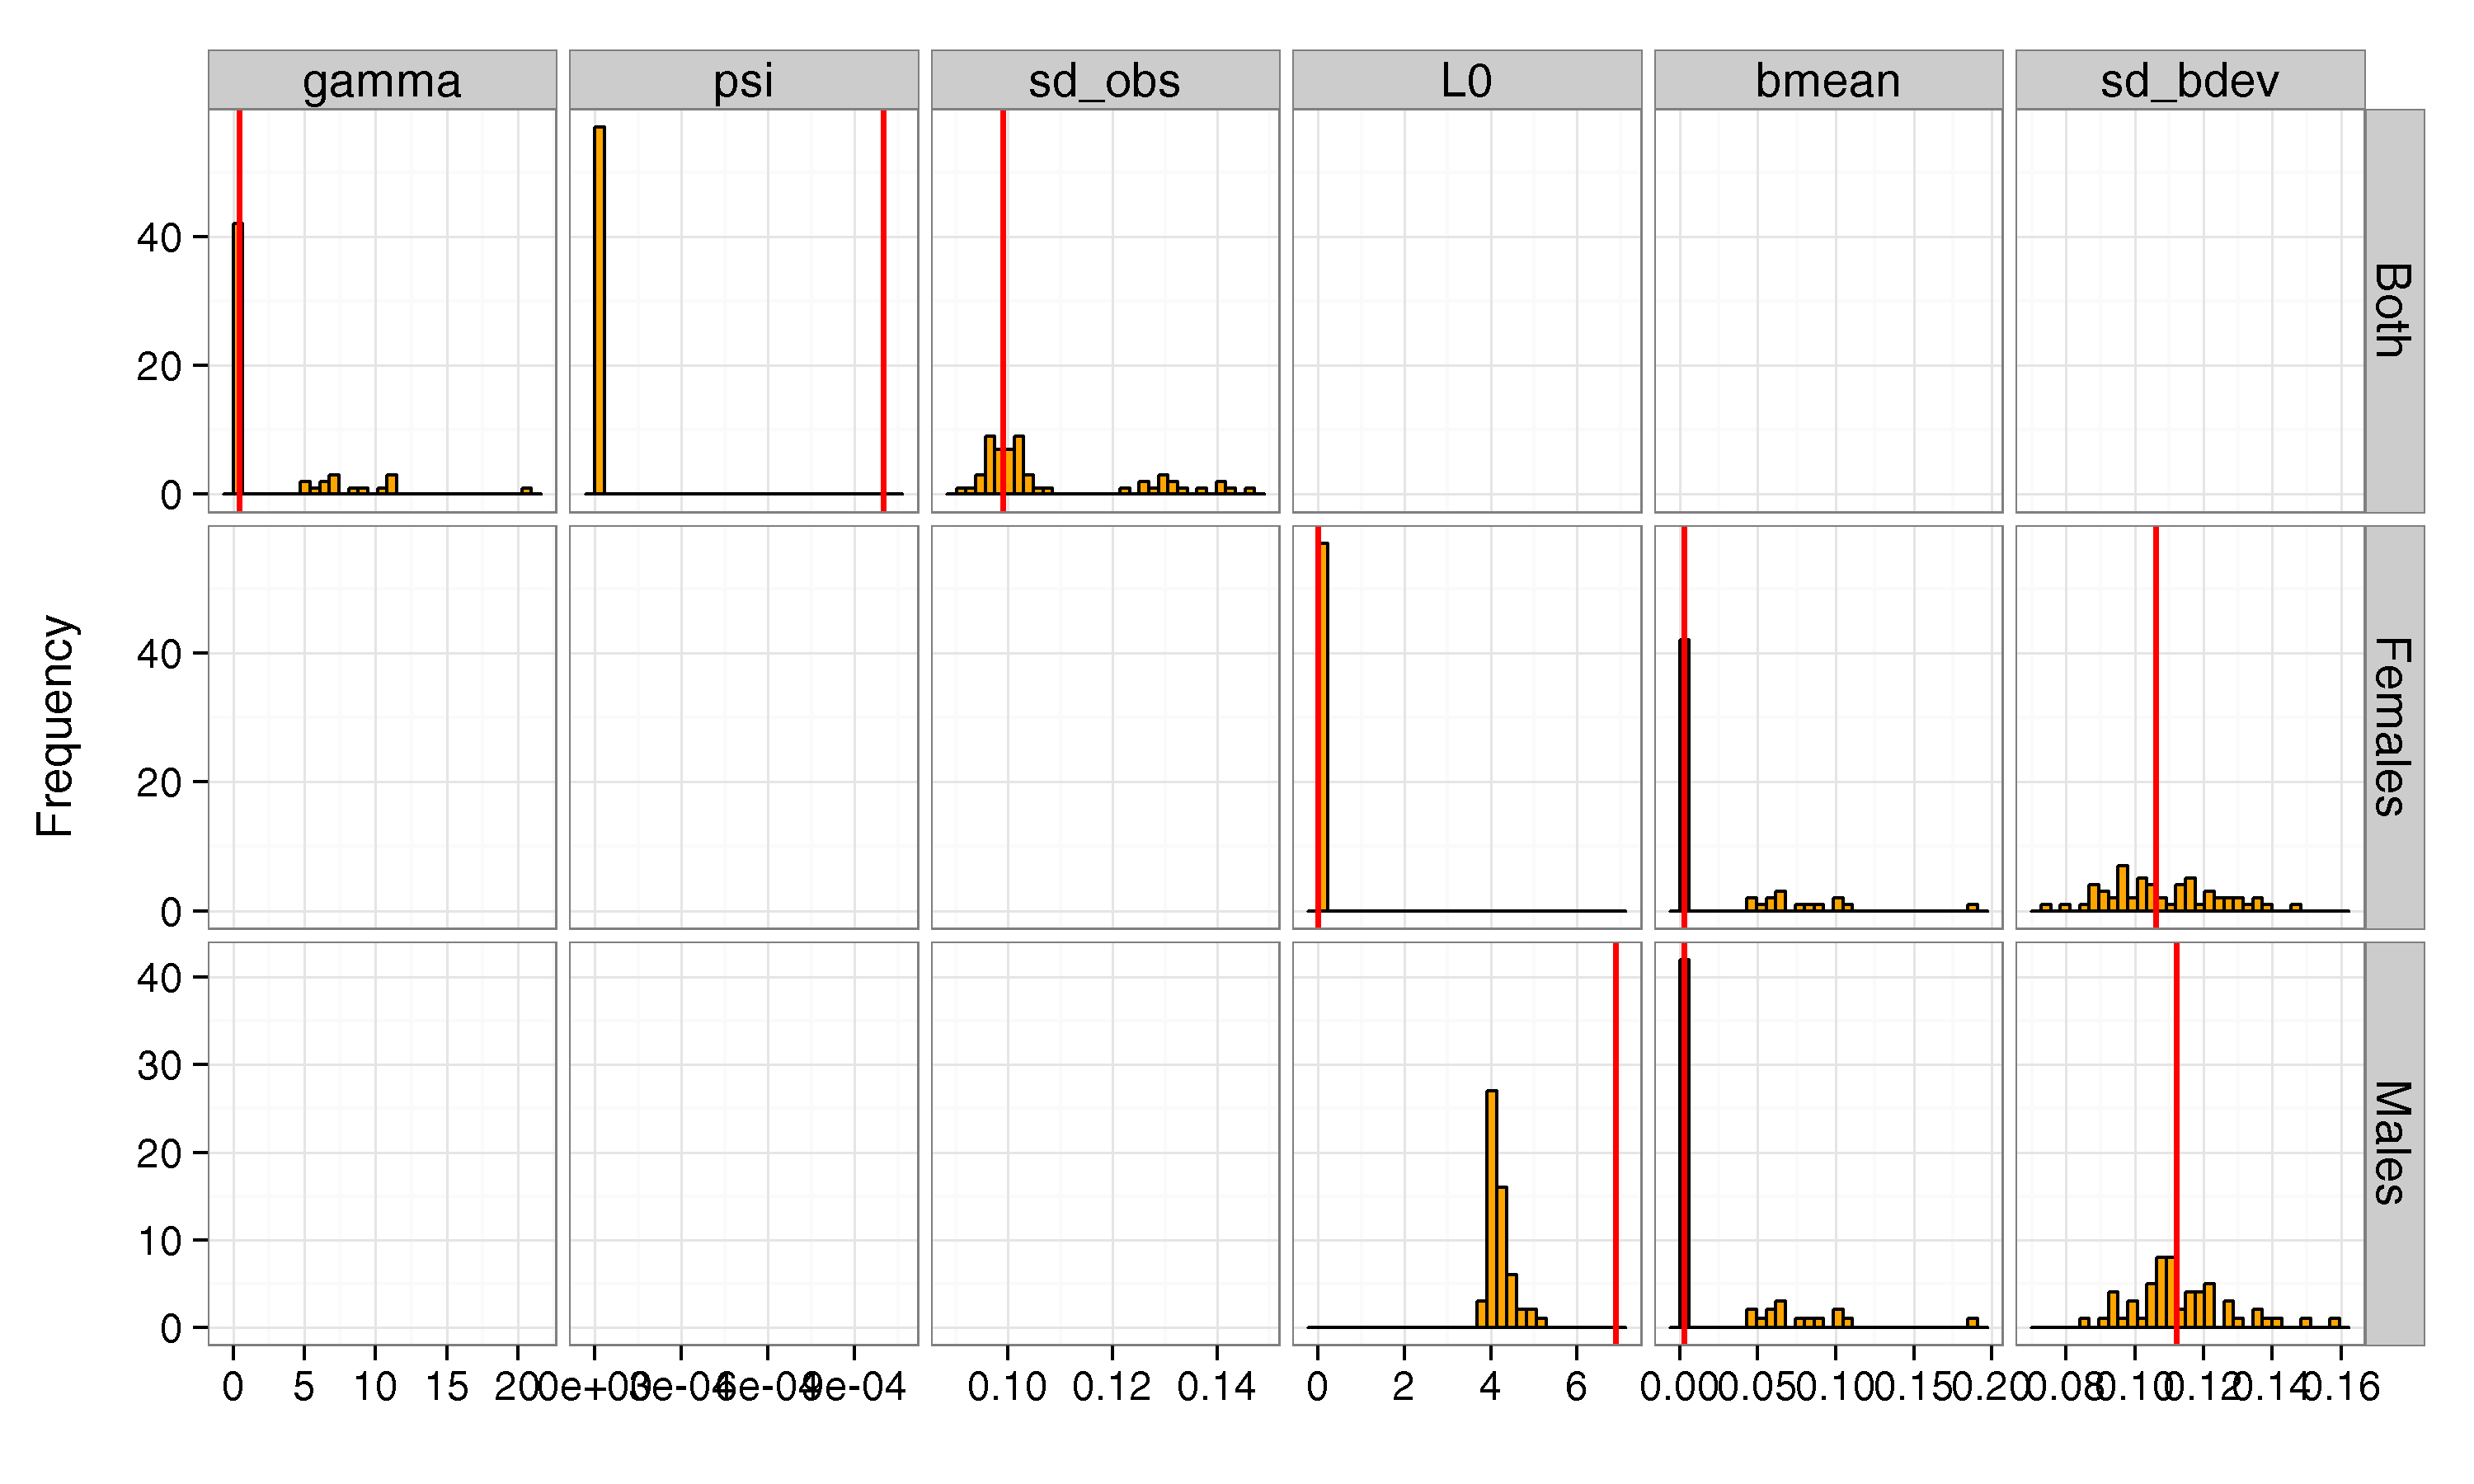
\includegraphics[width=\linewidth]{../simulation/sims2/results/SimPars.png}
  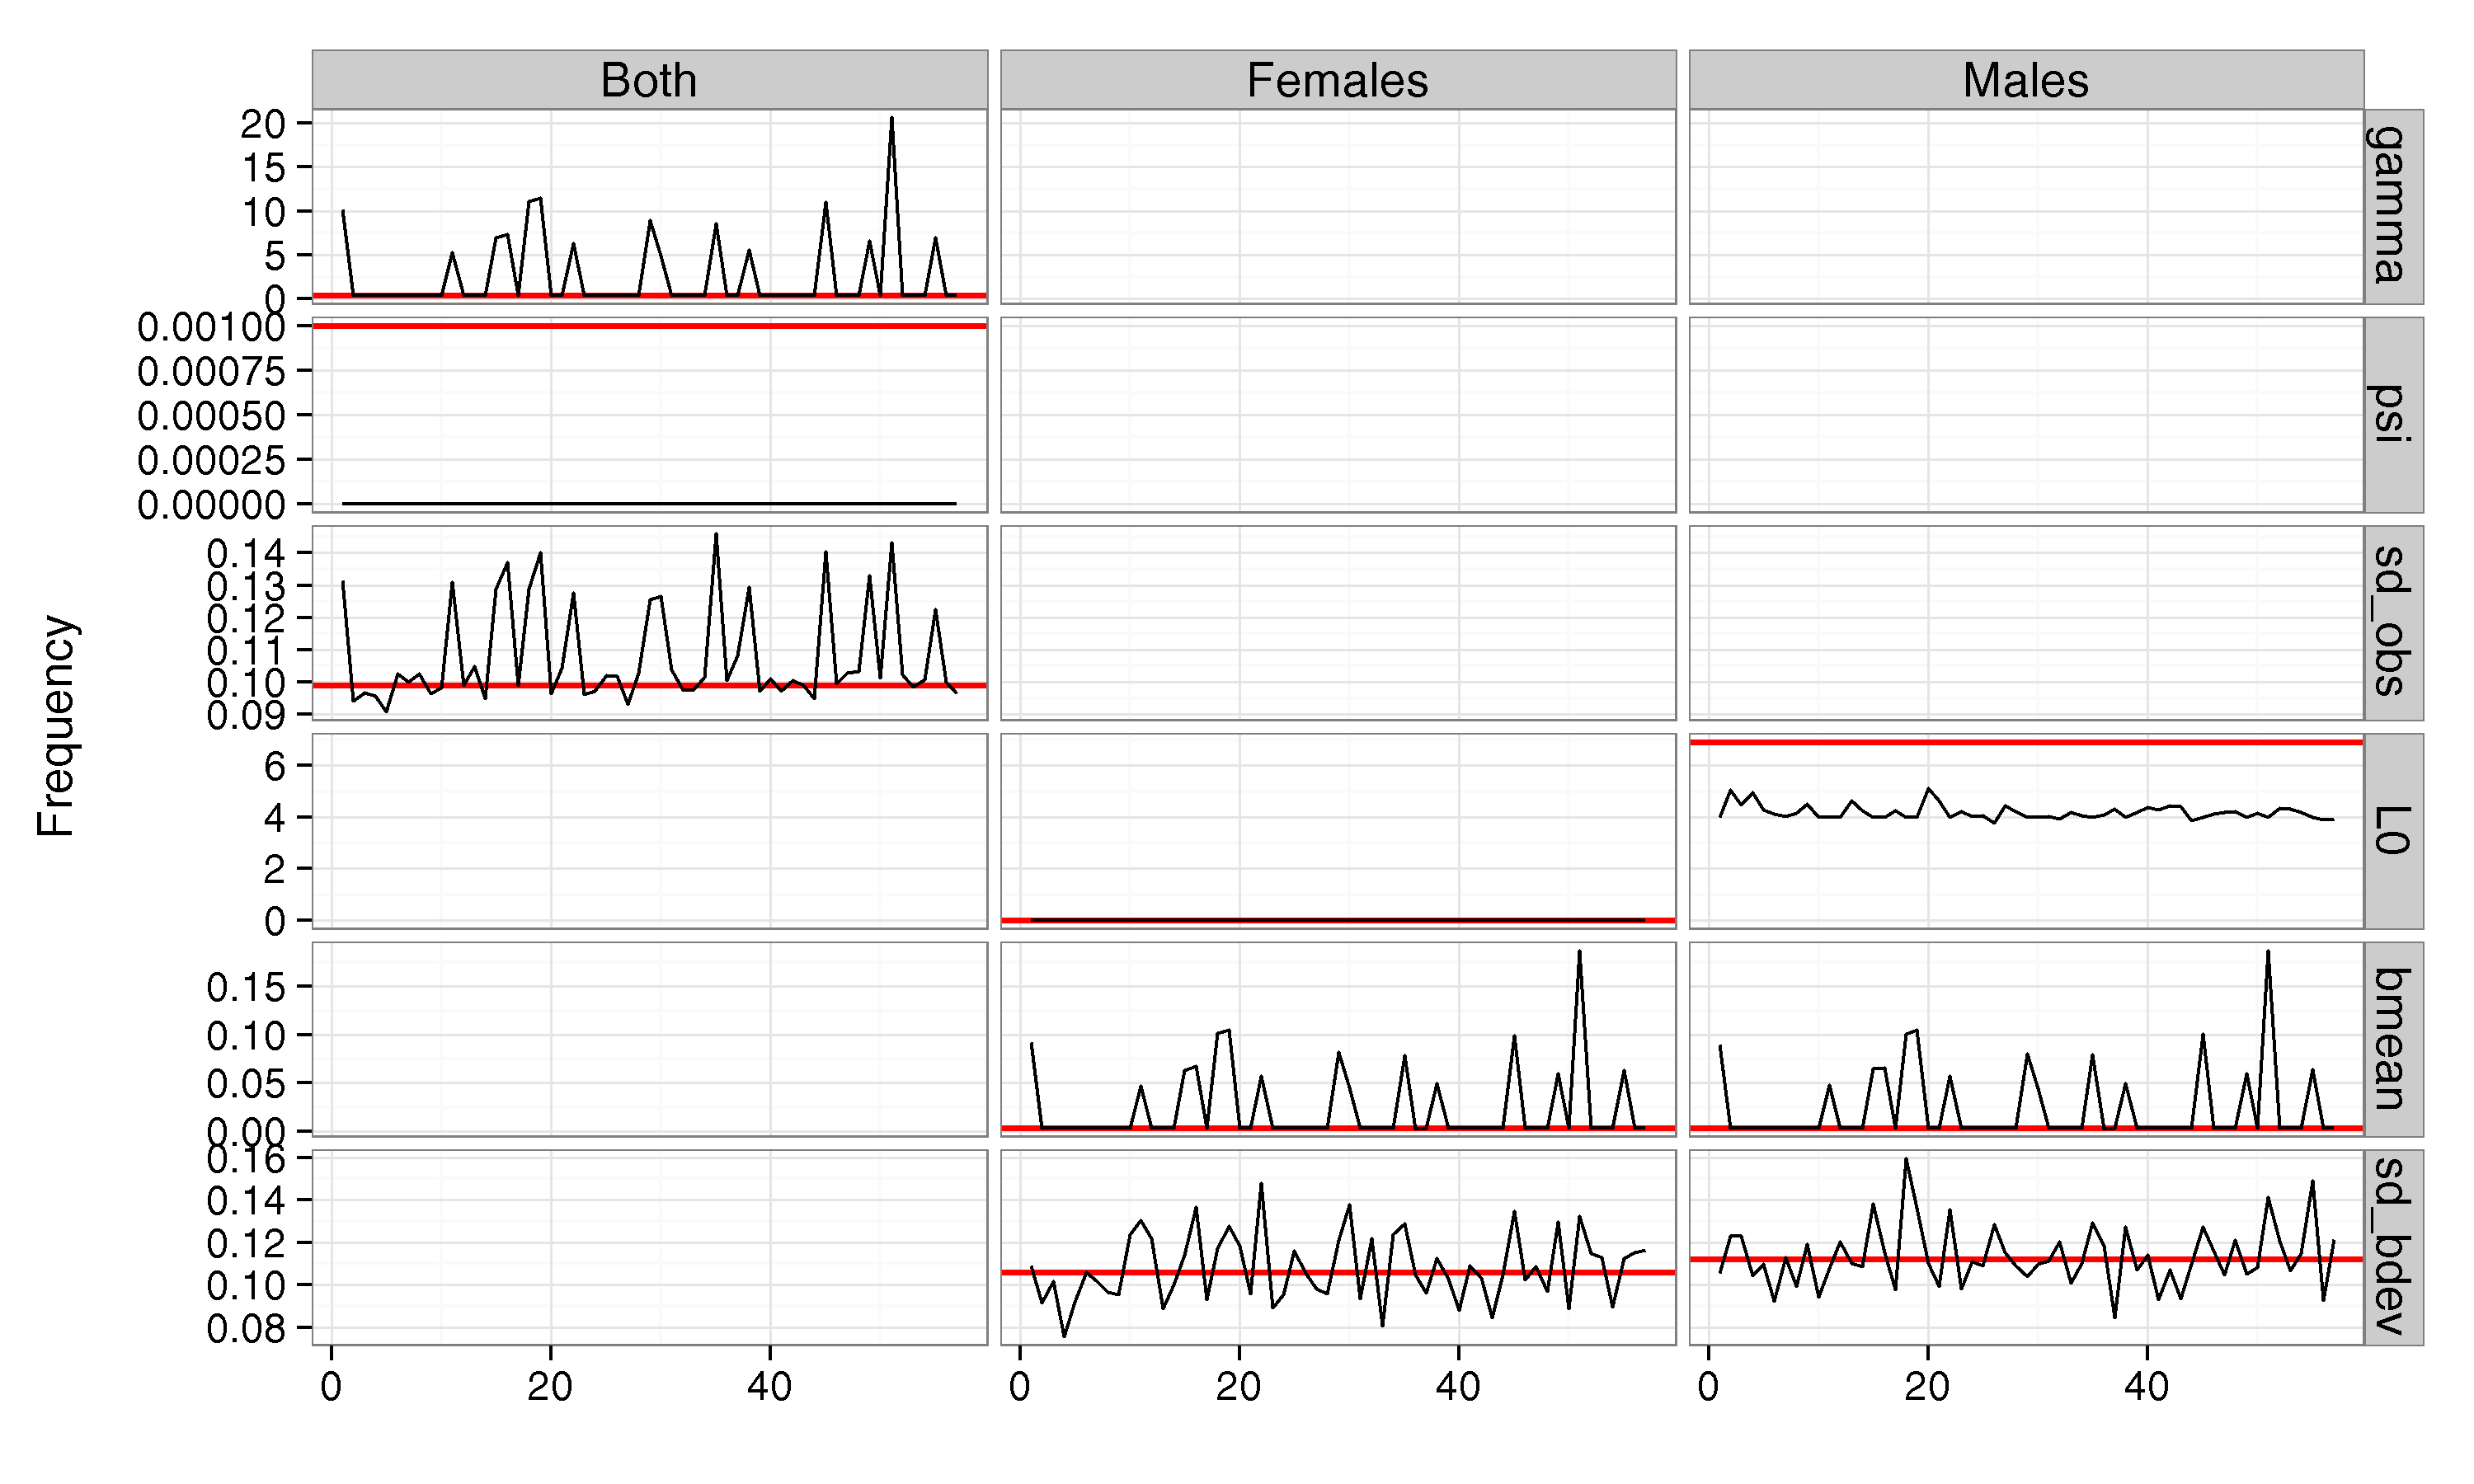
\includegraphics[width=\linewidth]{../simulation/sims2/results/TracePars.png}
  \begin{quote}
    \caption{pdH fits plotted only (57 of 100 fits were pdH).}
    \label{fig:sims2}
  \end{quote}
\end{figure}

\begin{figure}[!htbp]
  \centering
  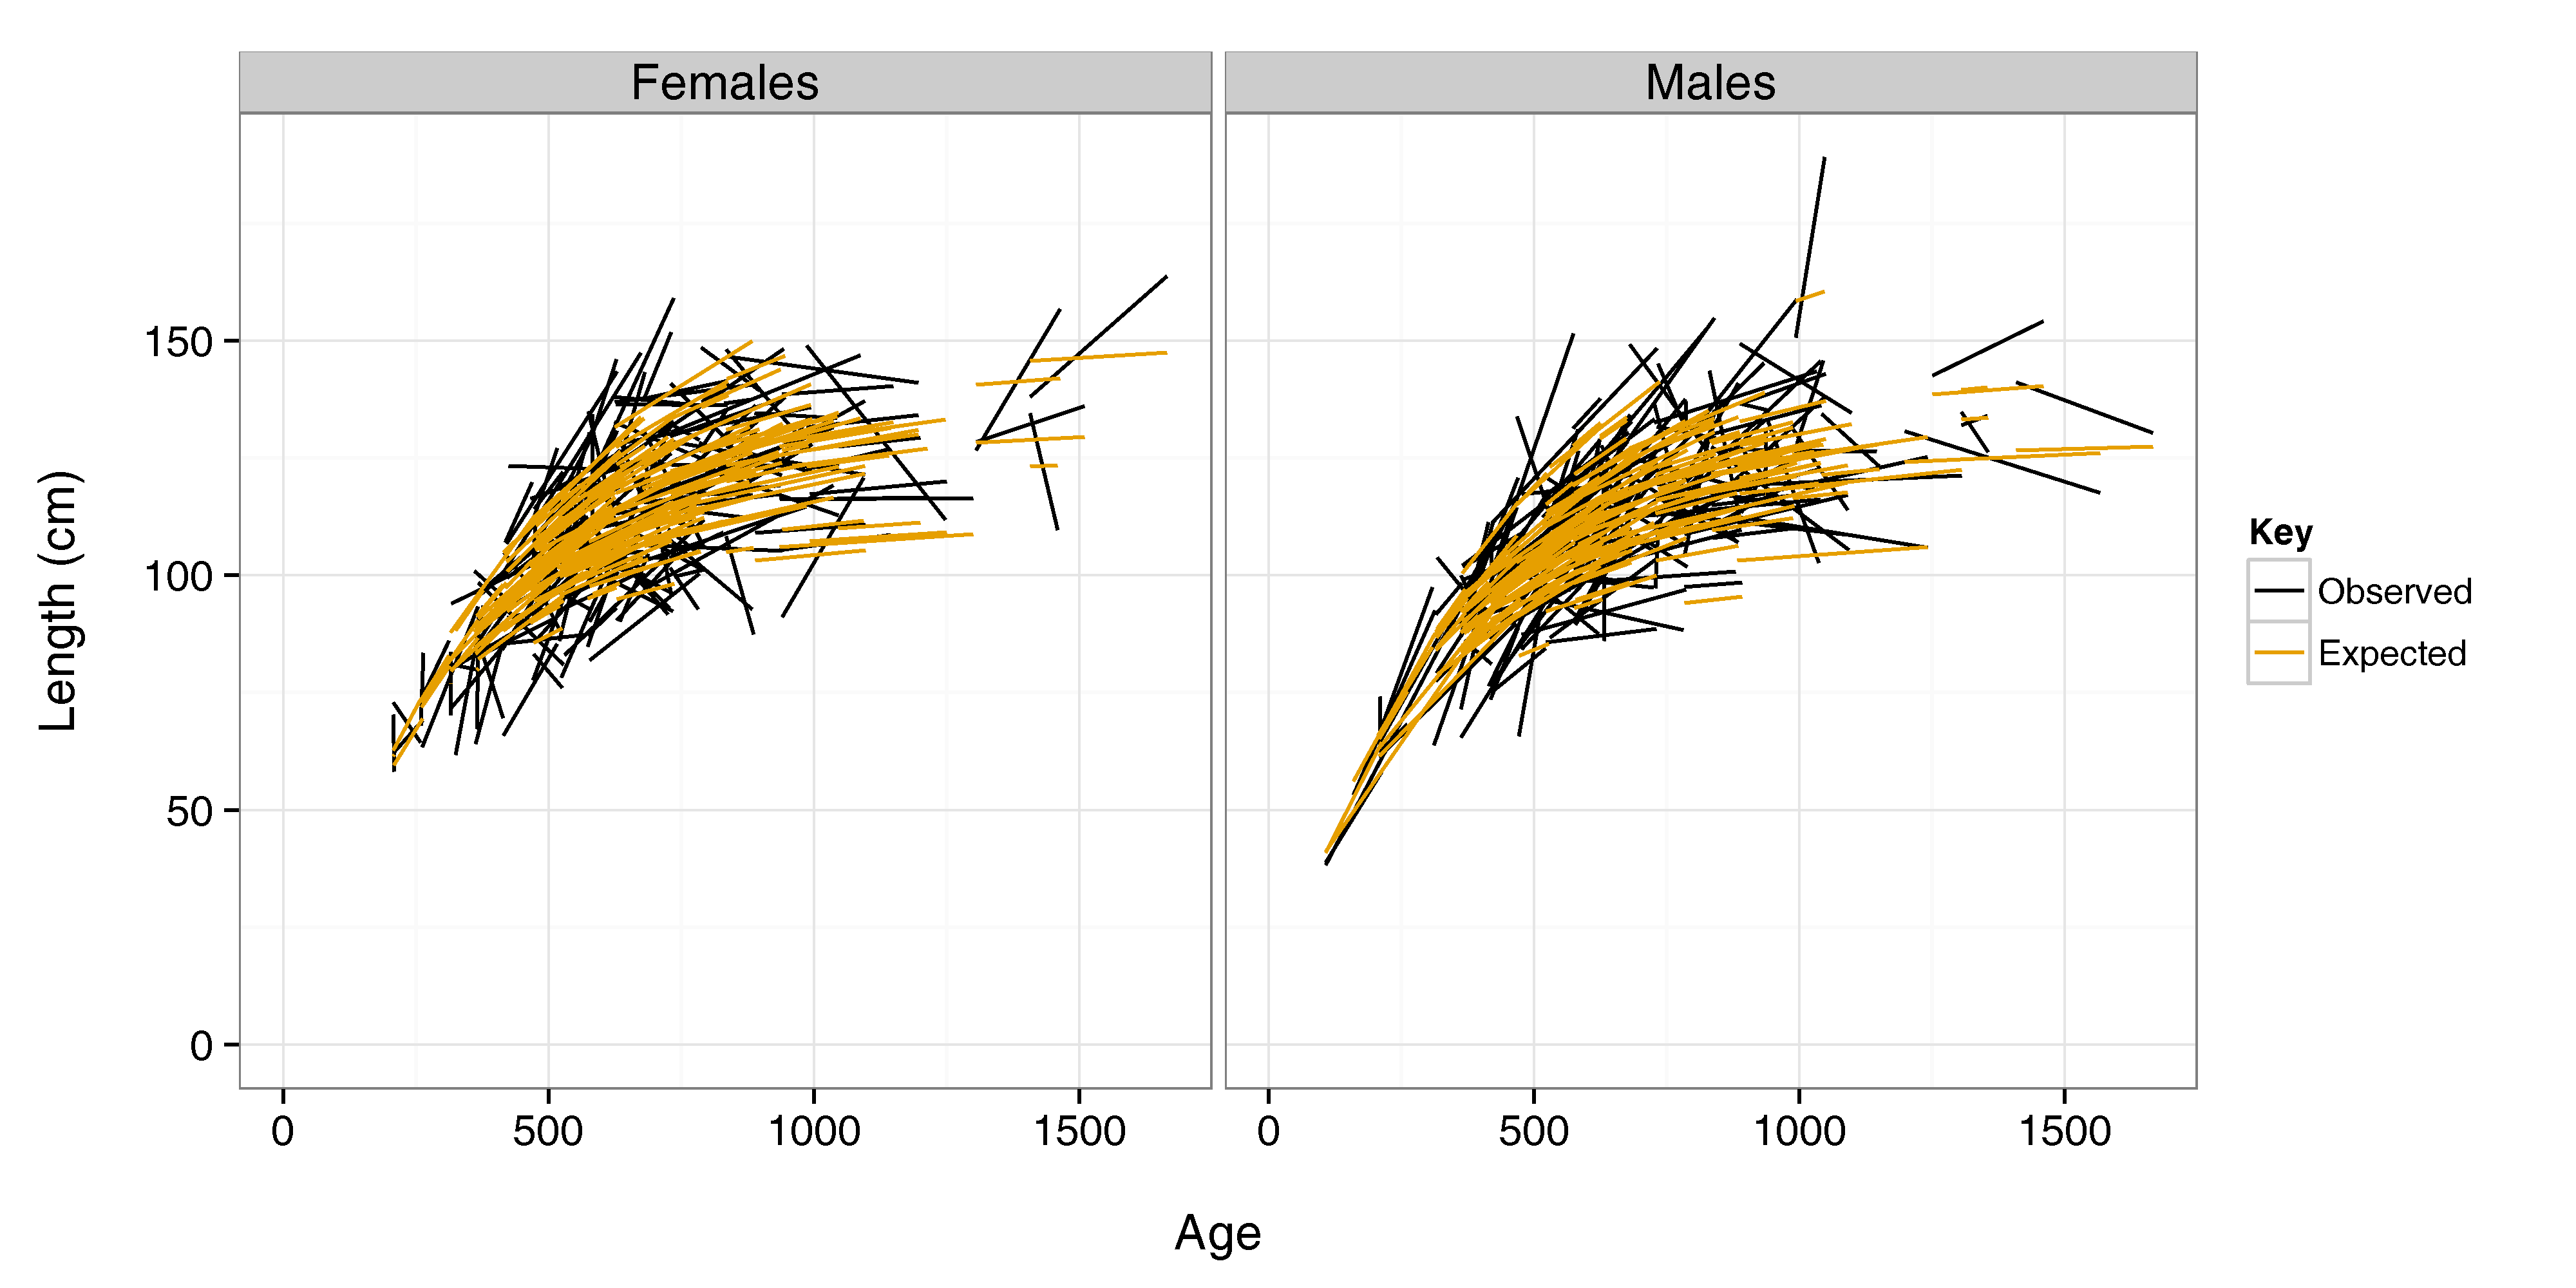
\includegraphics[width=\linewidth]{../simulation/sims2/results/IndivGrowth_3.png}
  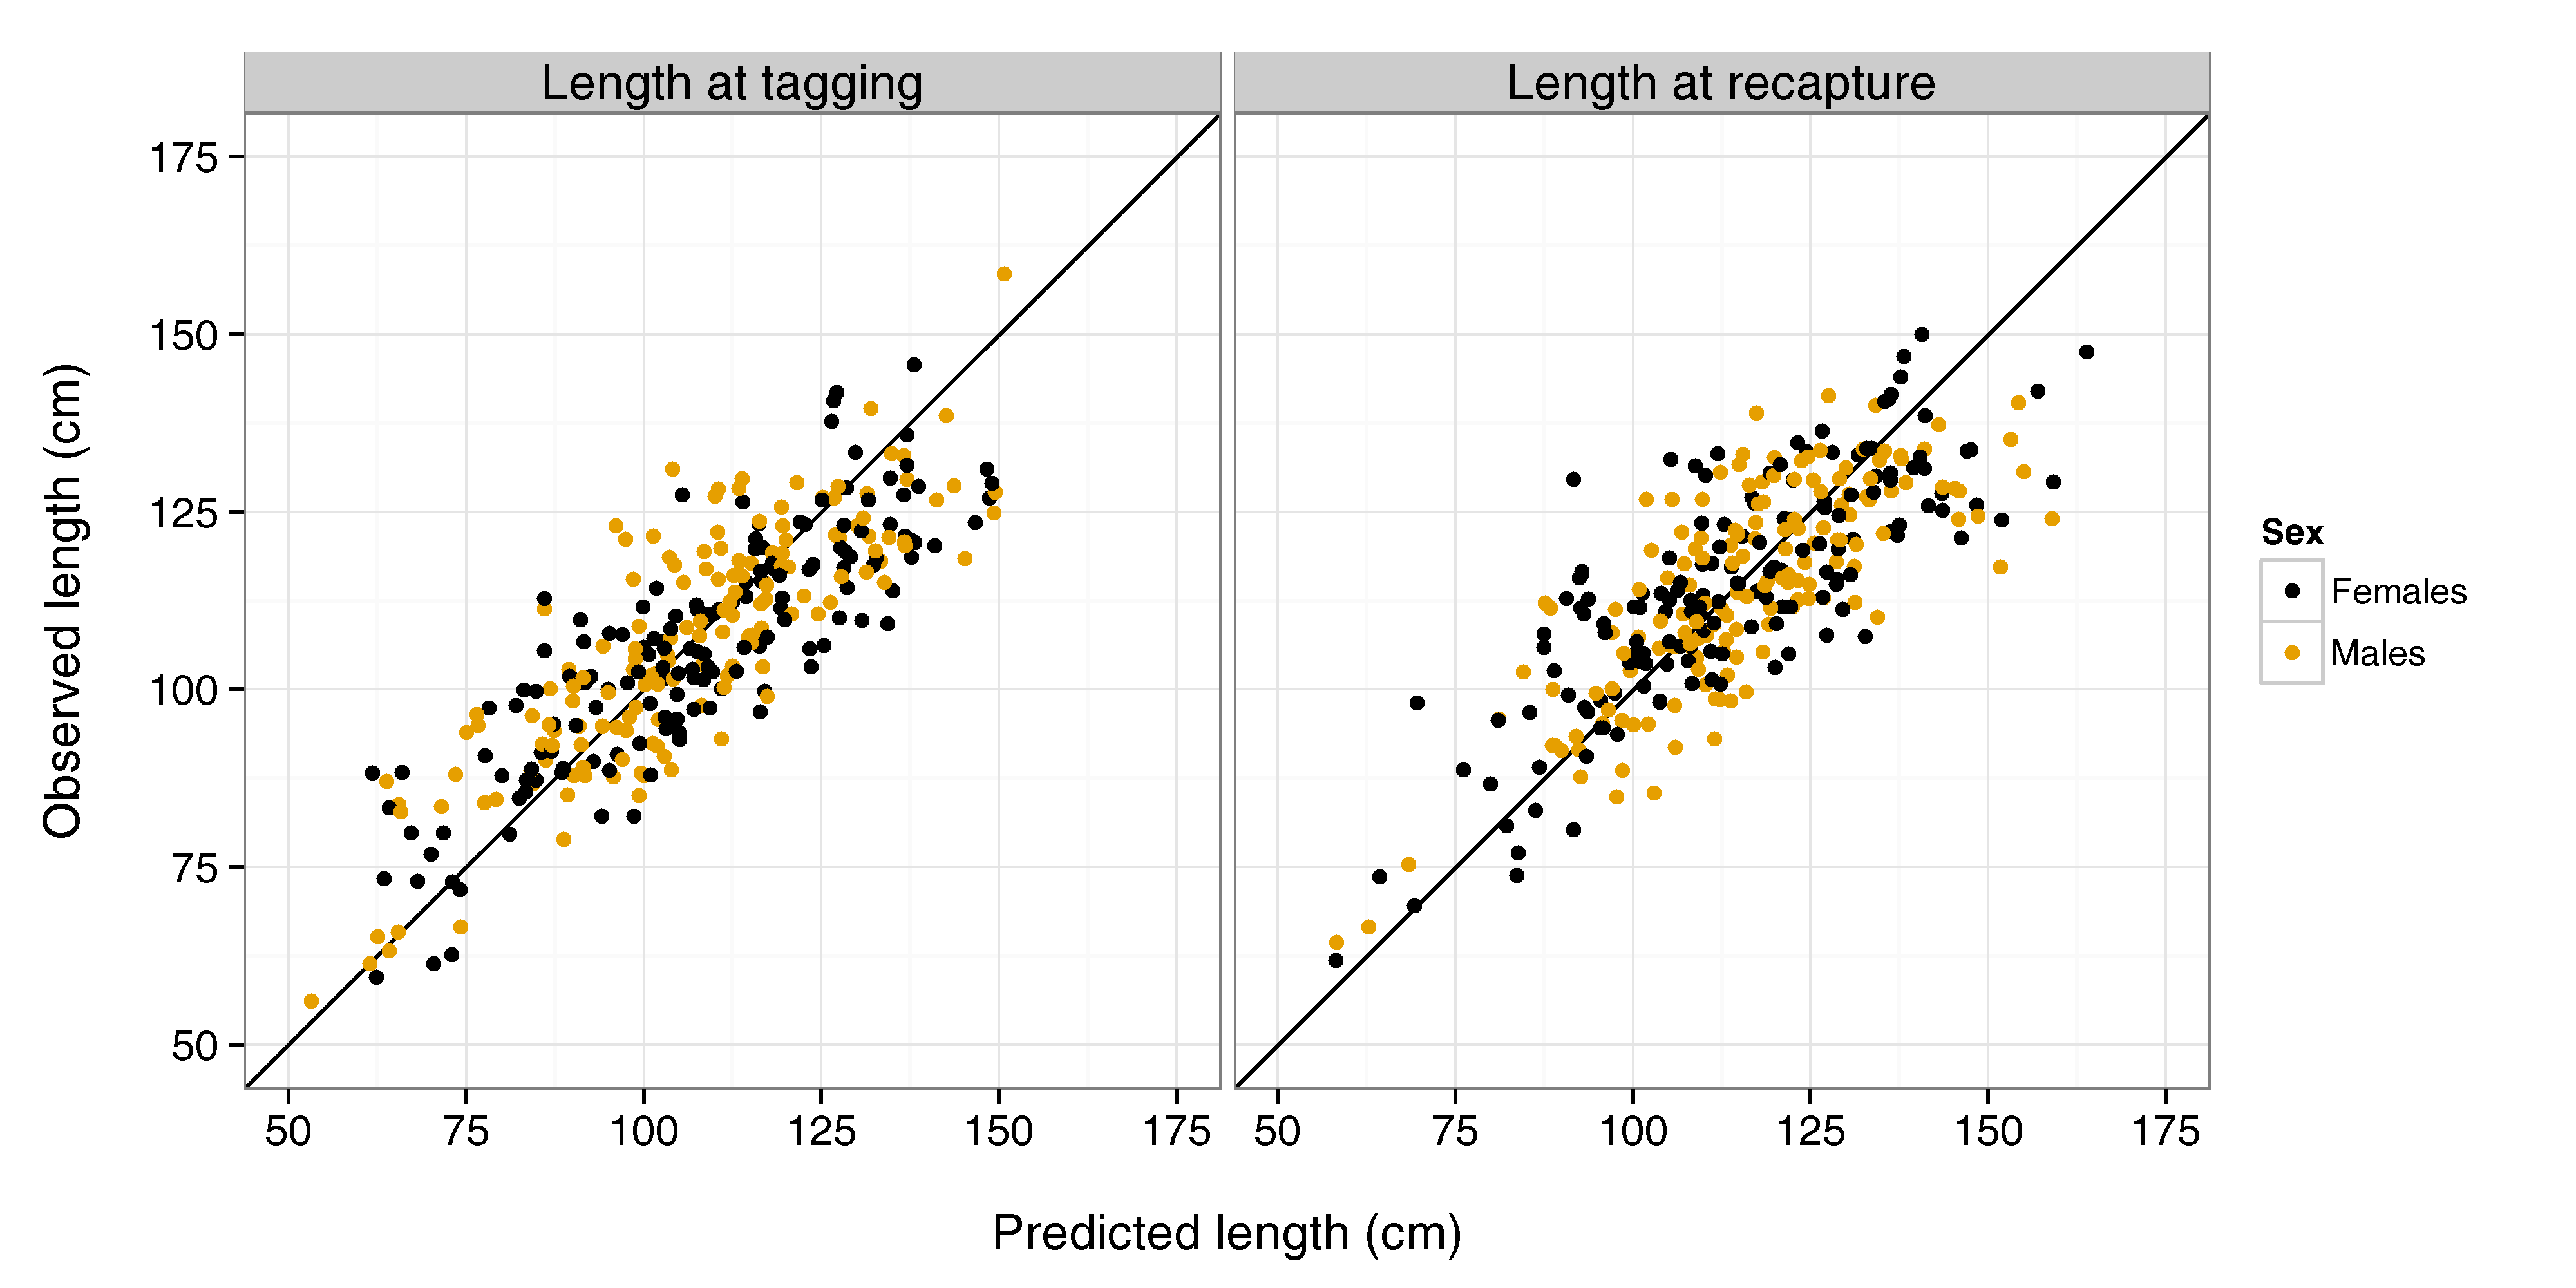
\includegraphics[width=\linewidth]{../simulation/sims2/results/ObsVsPred_3.png}
  \begin{quote}
    \caption{The first pdH simulation (sim 3).}
    \label{fig:sims2-fits}
  \end{quote}
\end{figure}



%%%%%%%%%%%%%%%%%%%%%%%%%%%%%%%%%%%%%%%%%%%%%%%%%%%%%%%%%%%%%%%%%%%%%%%%%%%%%%%%%

%\bibliographystyle{agsm}
%\bibliography{refs/myrefs}

%%%%%%%%%%%%%%%%%%%%%%%%%%%%%%%%%%%%%%%%%%%%%%%%%%%%%%%%%%%%%%%%%%%%%%%%%%%%%%%%%

\end{document}




I also tried this:
\begin{itemize}
\item Sampled sex using a binomial distribution.
\item Fit lognormal distributions to Age1 and time at liberty and simulate
  independently from the distributions.
\item Calculate Age2 given Age1 and time at liberty.
\item Rounded Age1, Age2 and time at liberty off to the nearest integer.
\end{itemize}
But this resulted in unrealistic Age2's (i.e. when a long time at liberty is
added to an already old fish), the plots just looked a bit silly.

Below are some exmaple plots using the first sampling approach above then
running these through our simulation model. 
\begin{figure}[!htbp]
  \centering
  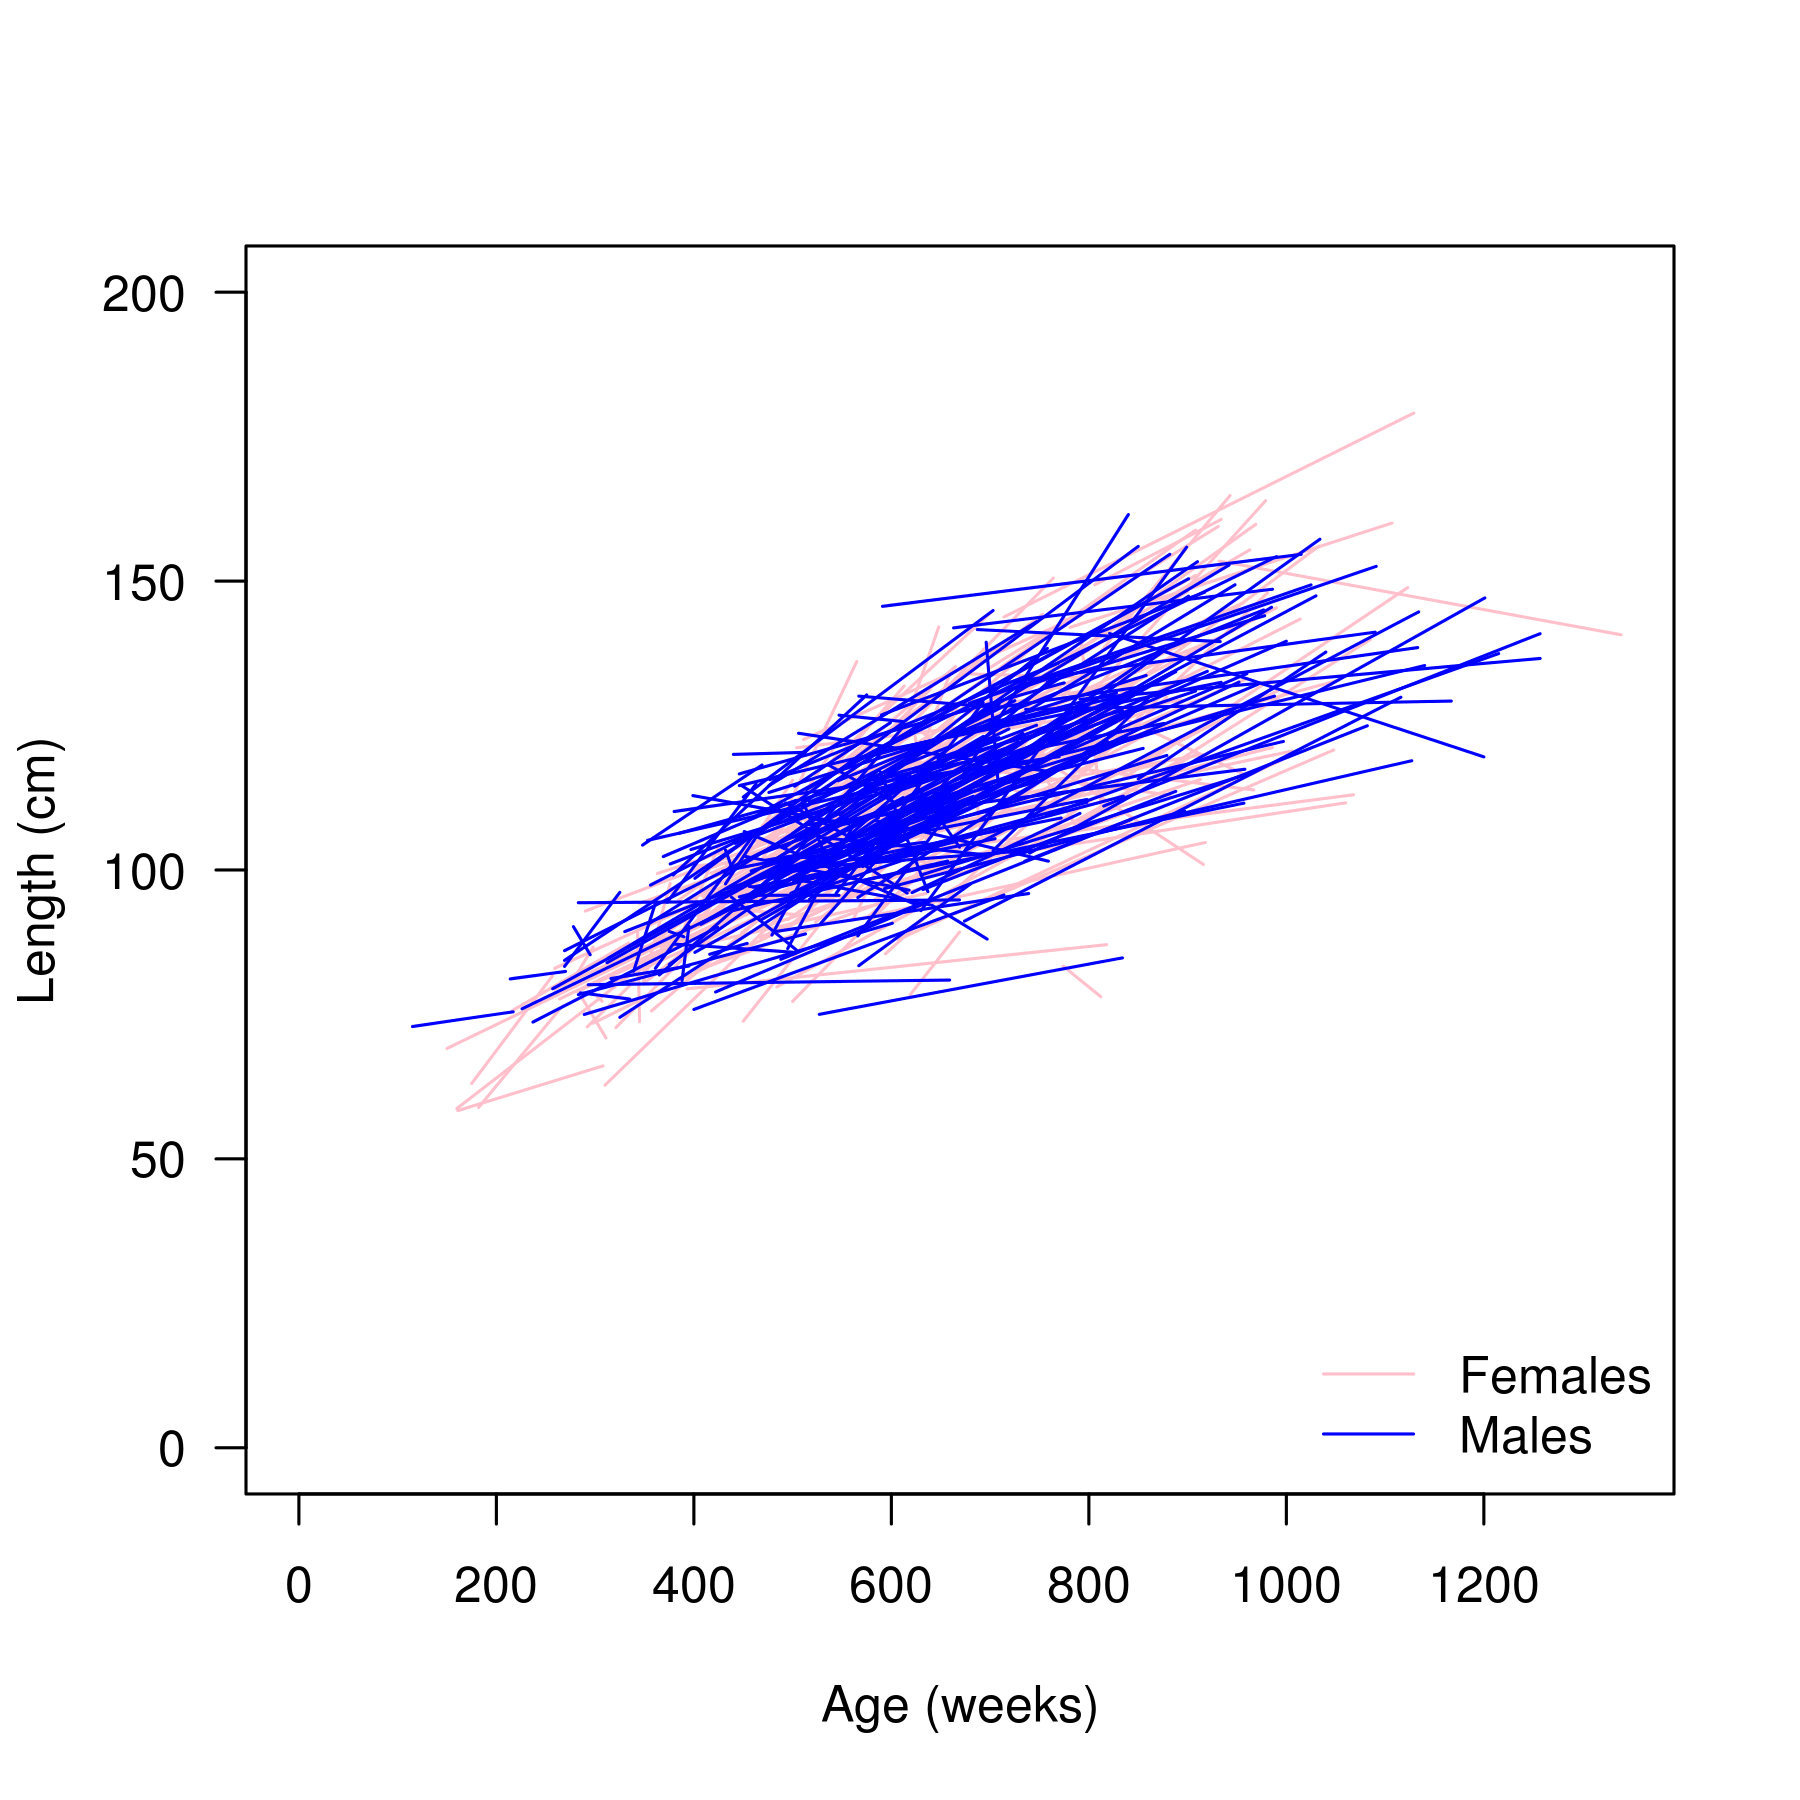
\includegraphics[width=0.49\linewidth]{../simulation/sims/growth-1.png}
  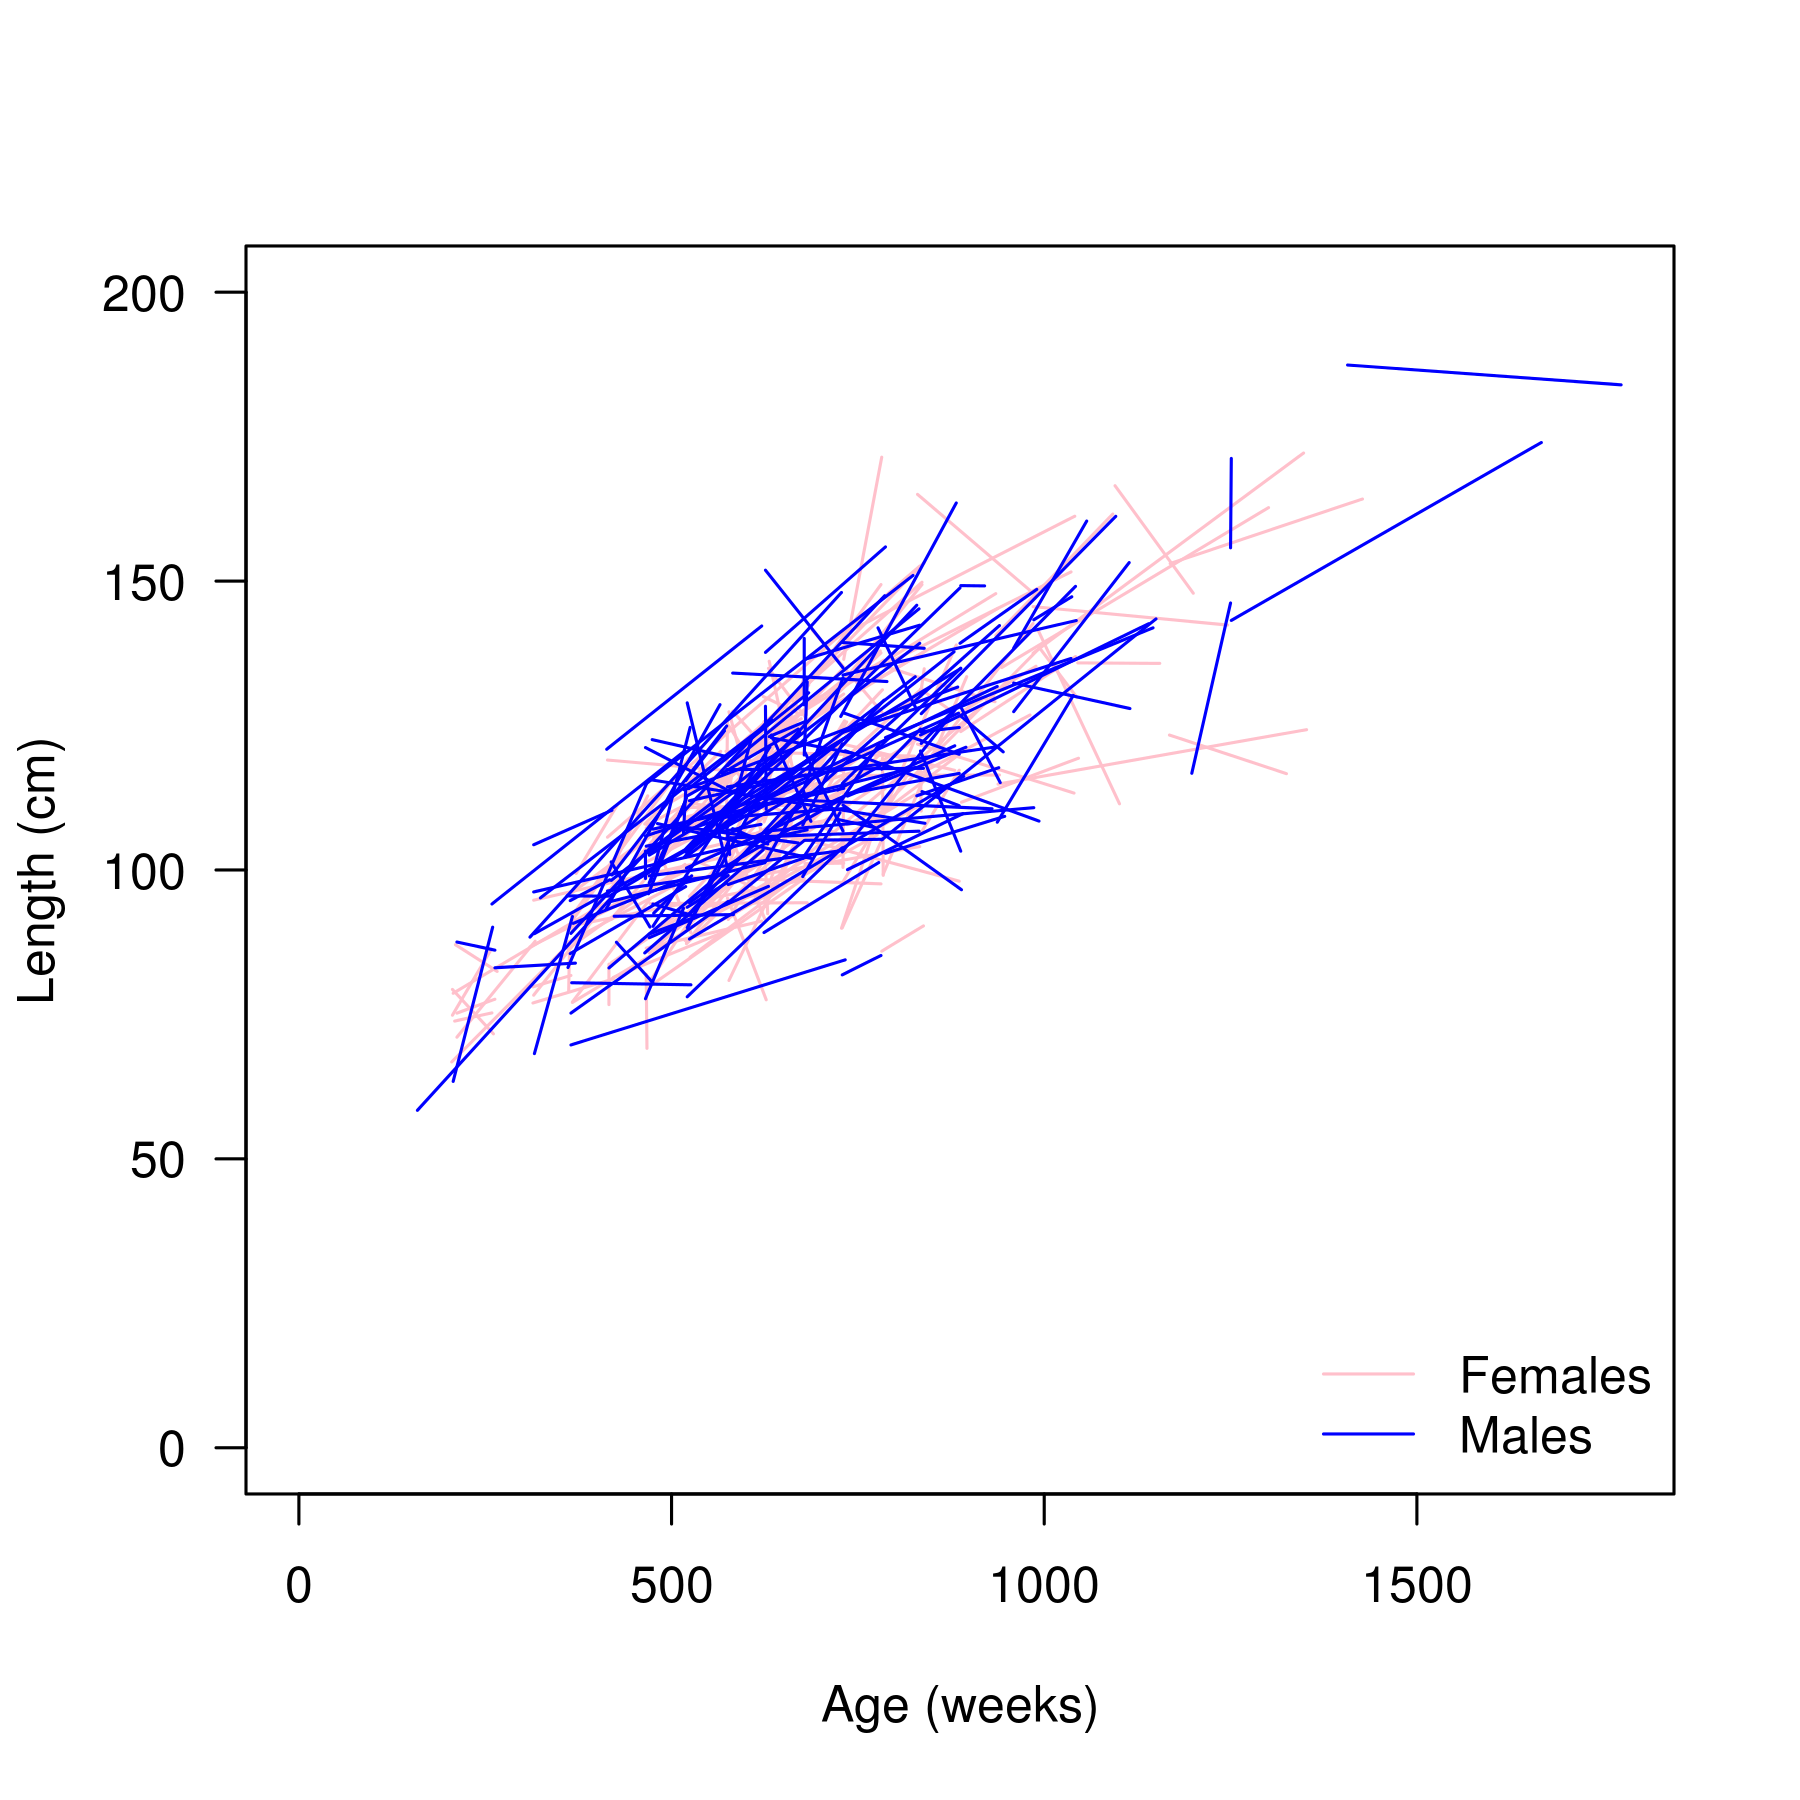
\includegraphics[width=0.49\linewidth]{../simulation/sims/growth-2.png}
  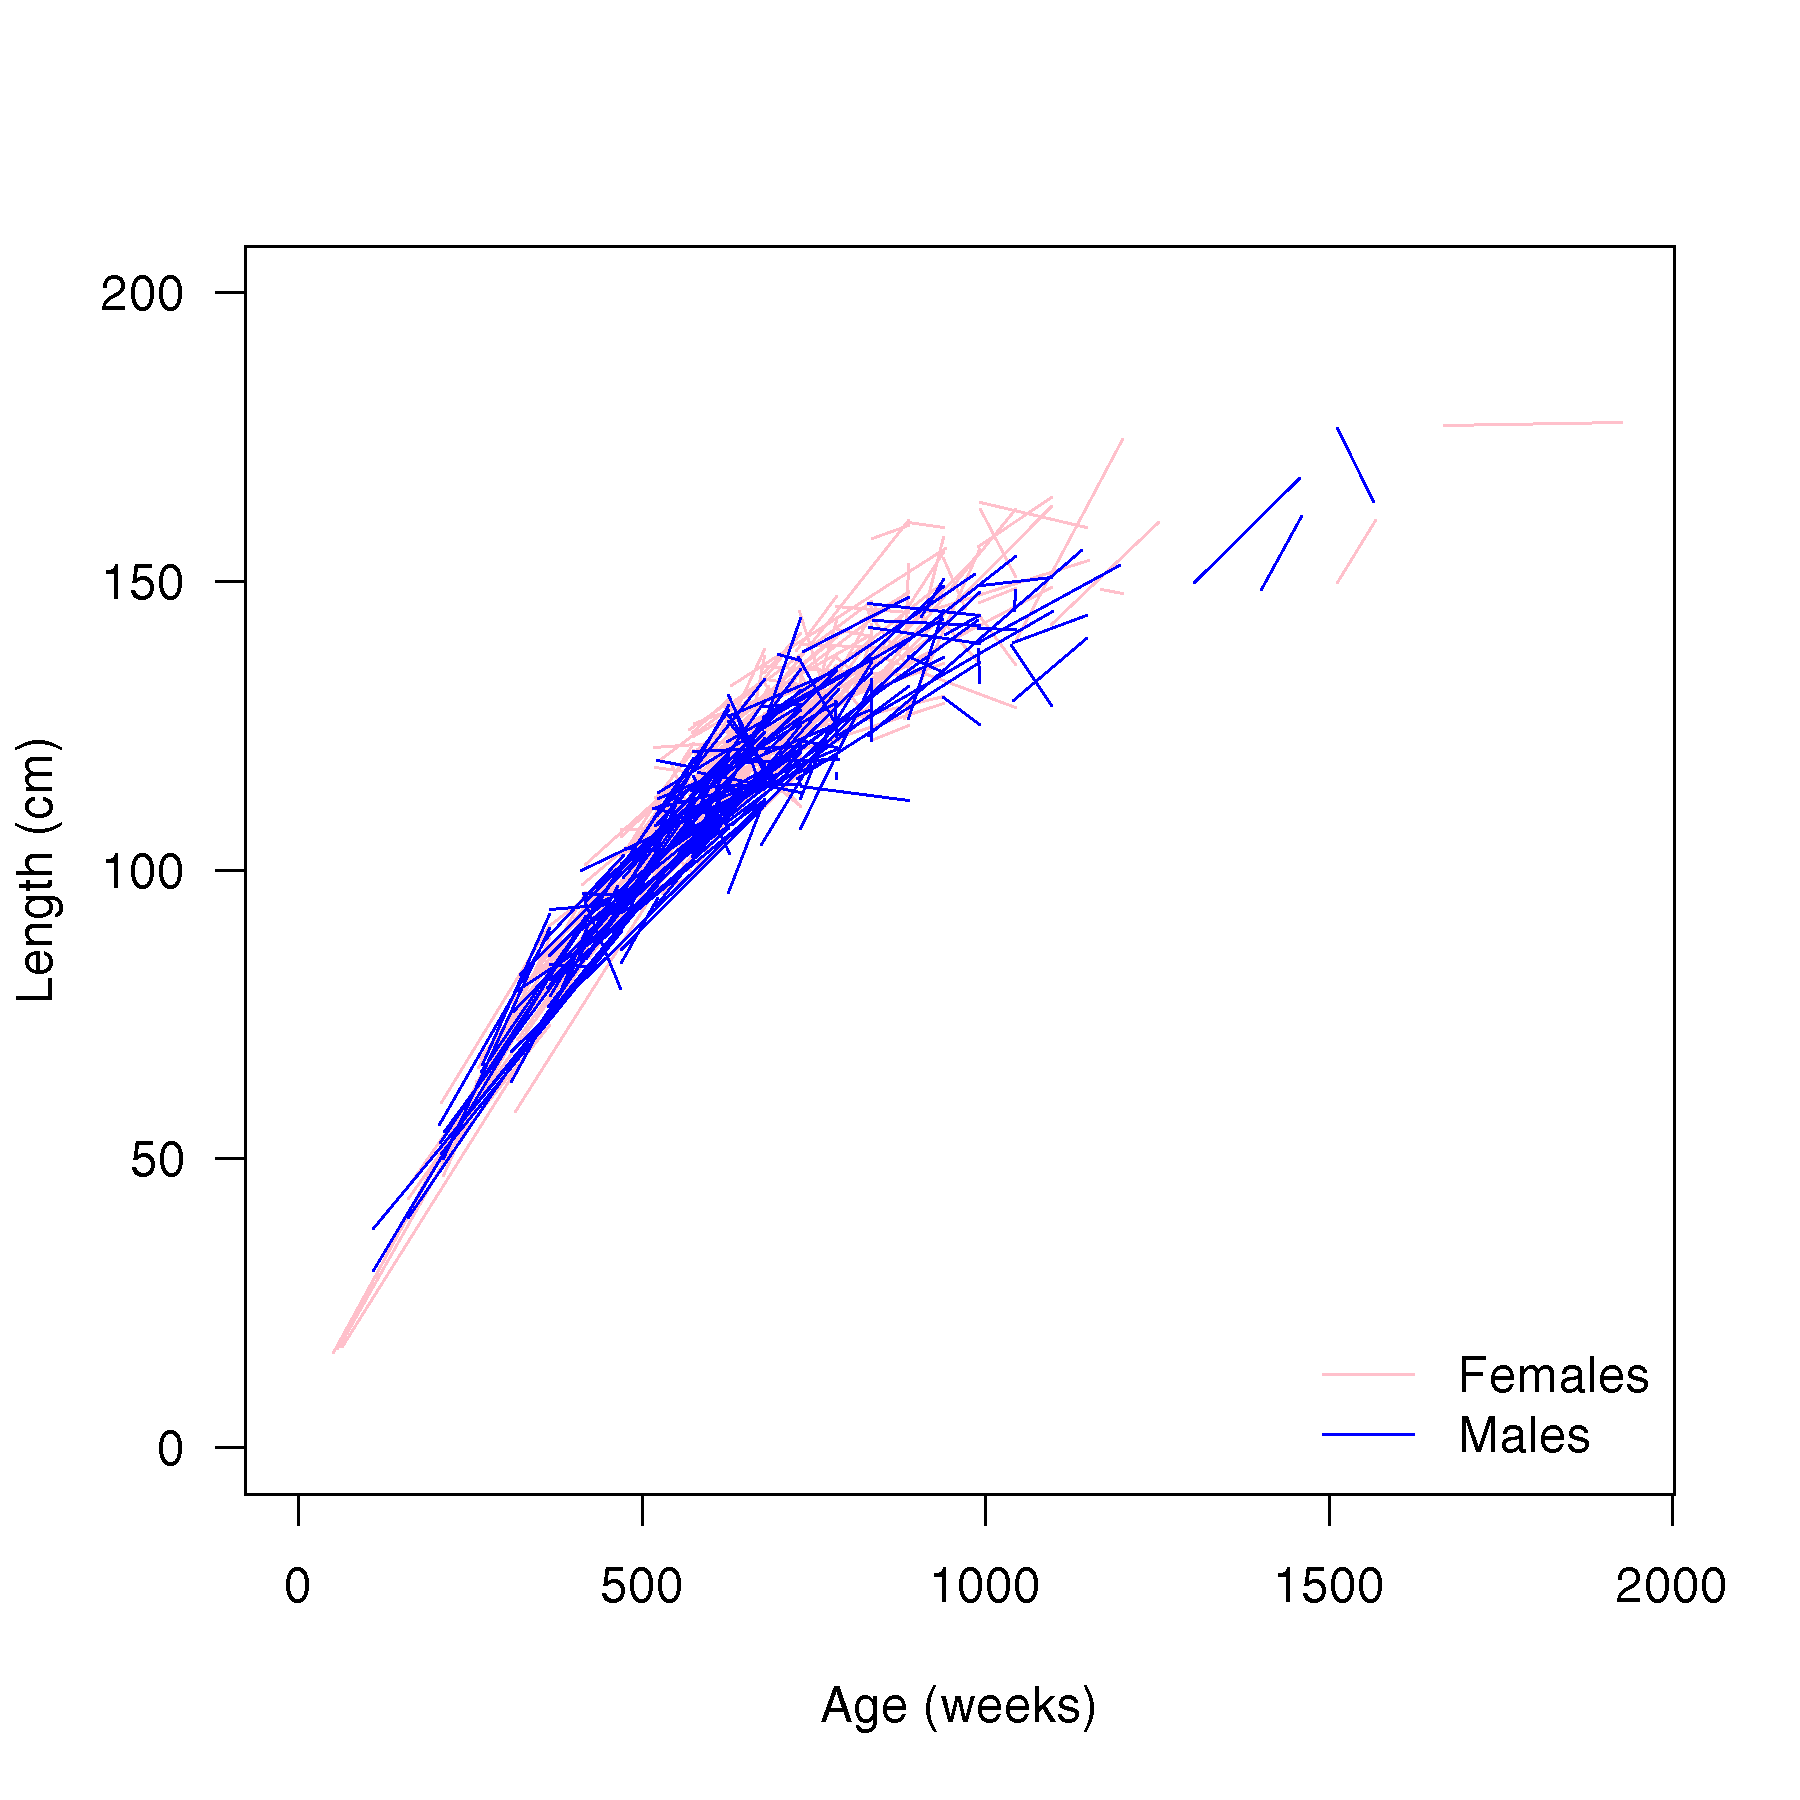
\includegraphics[width=0.49\linewidth]{../simulation/sims/growth-6.png}
  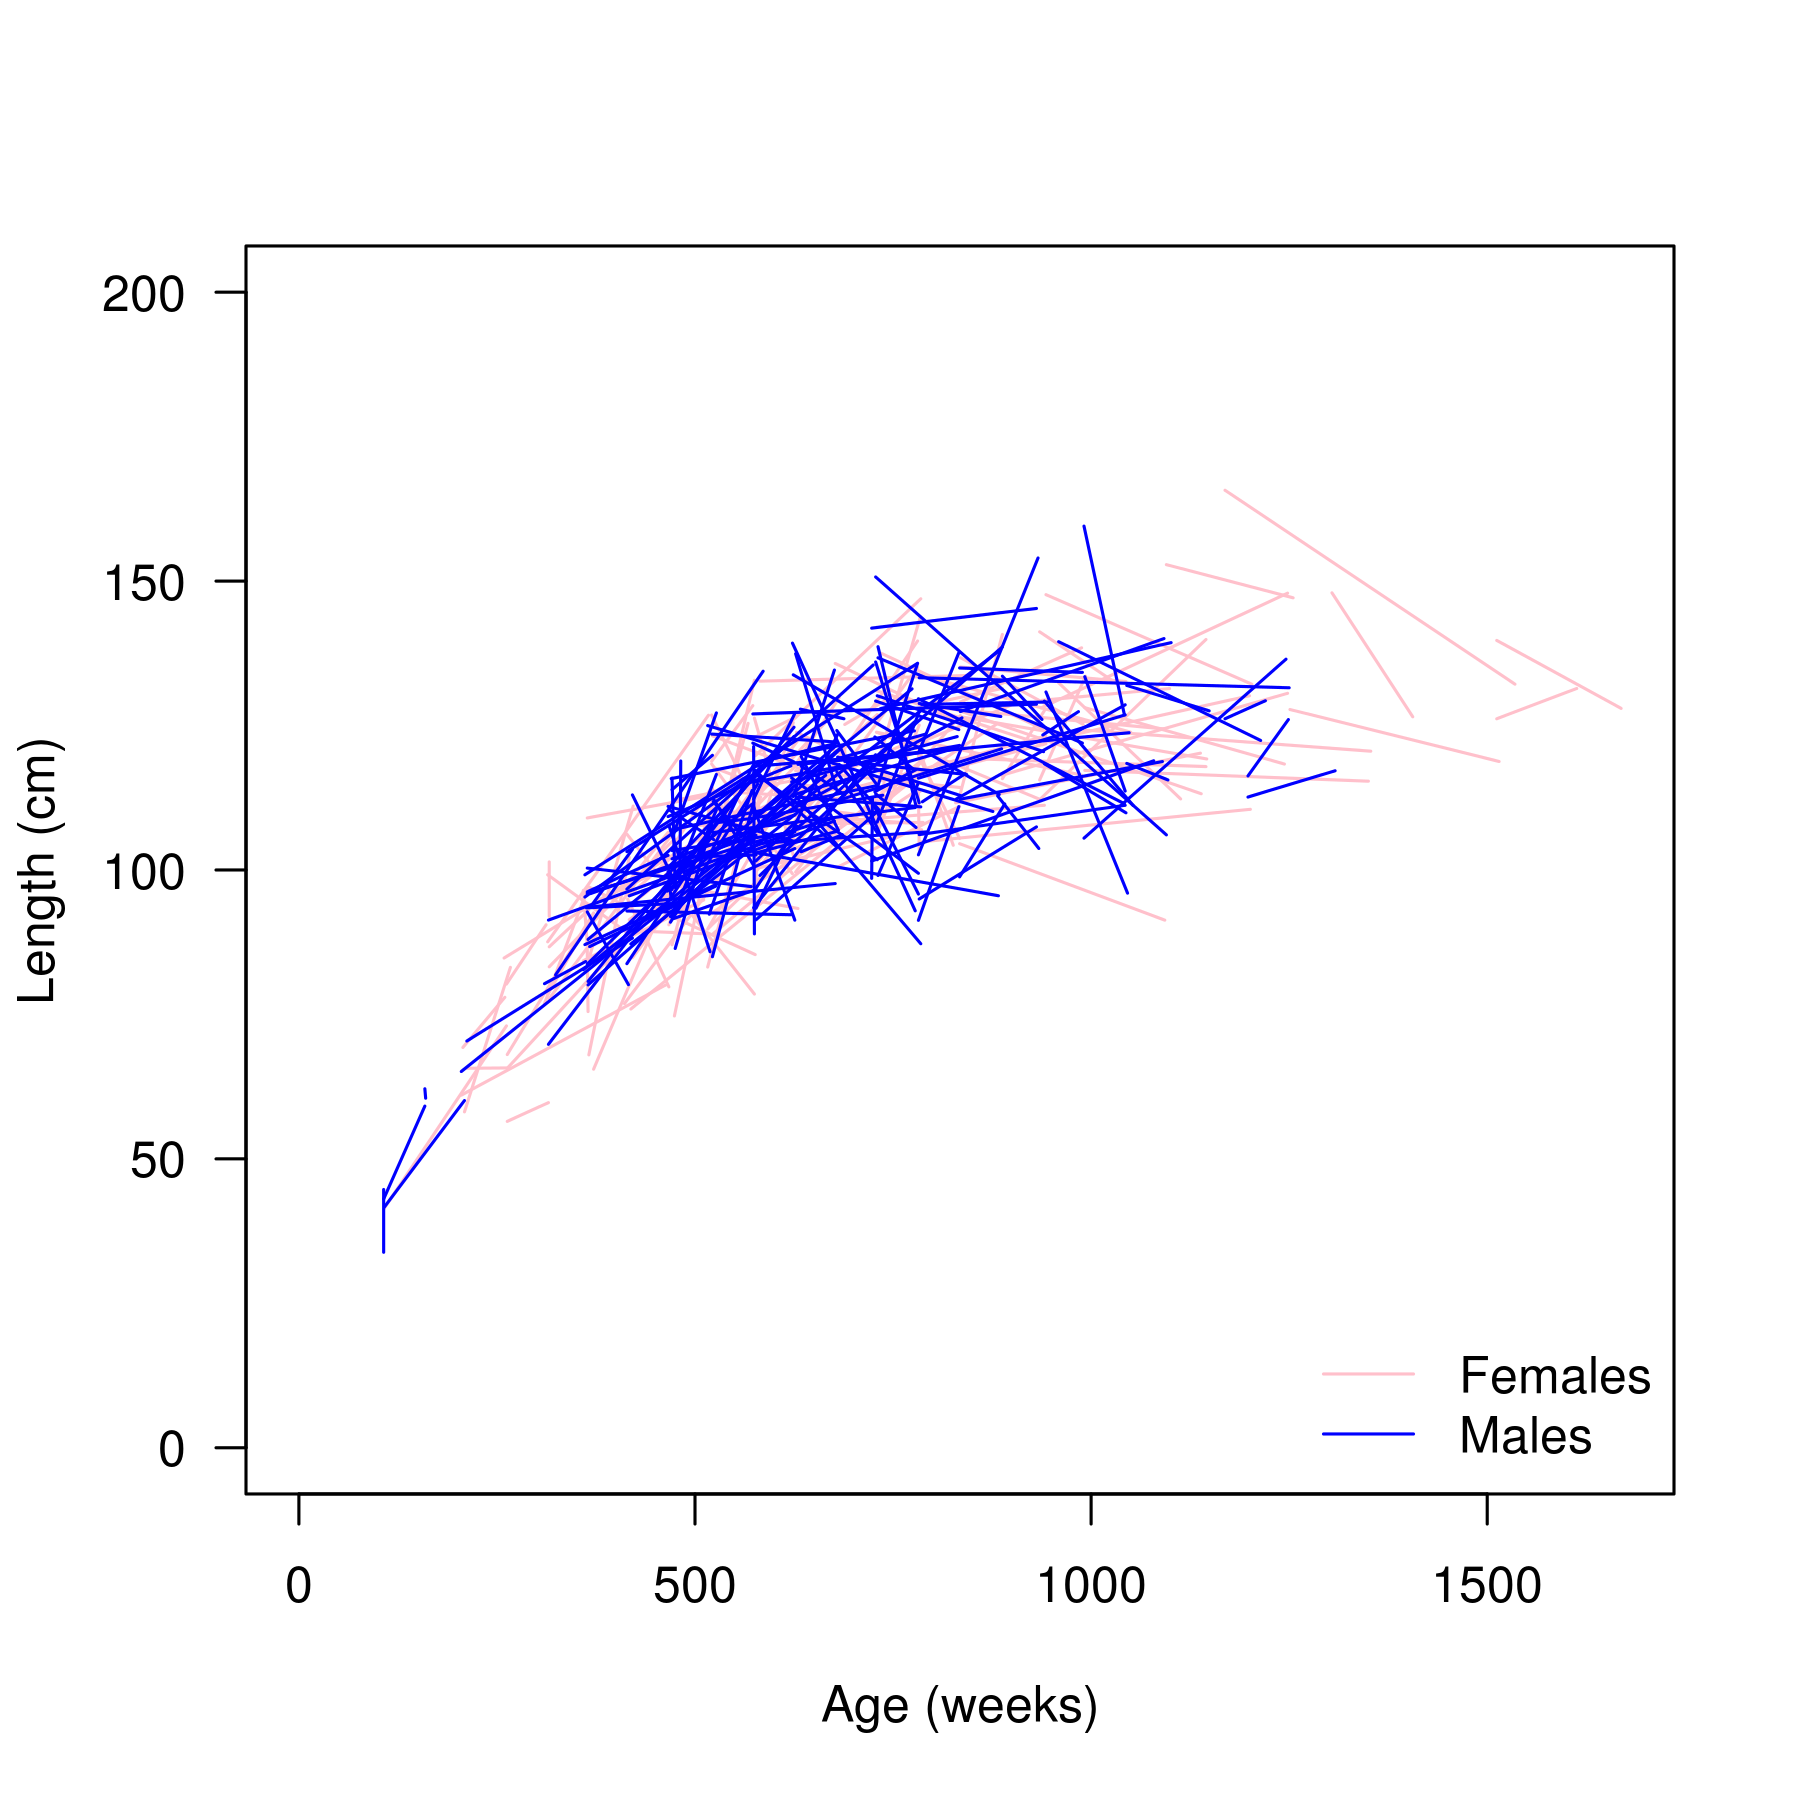
\includegraphics[width=0.49\linewidth]{../simulation/sims/growth-45.png}
  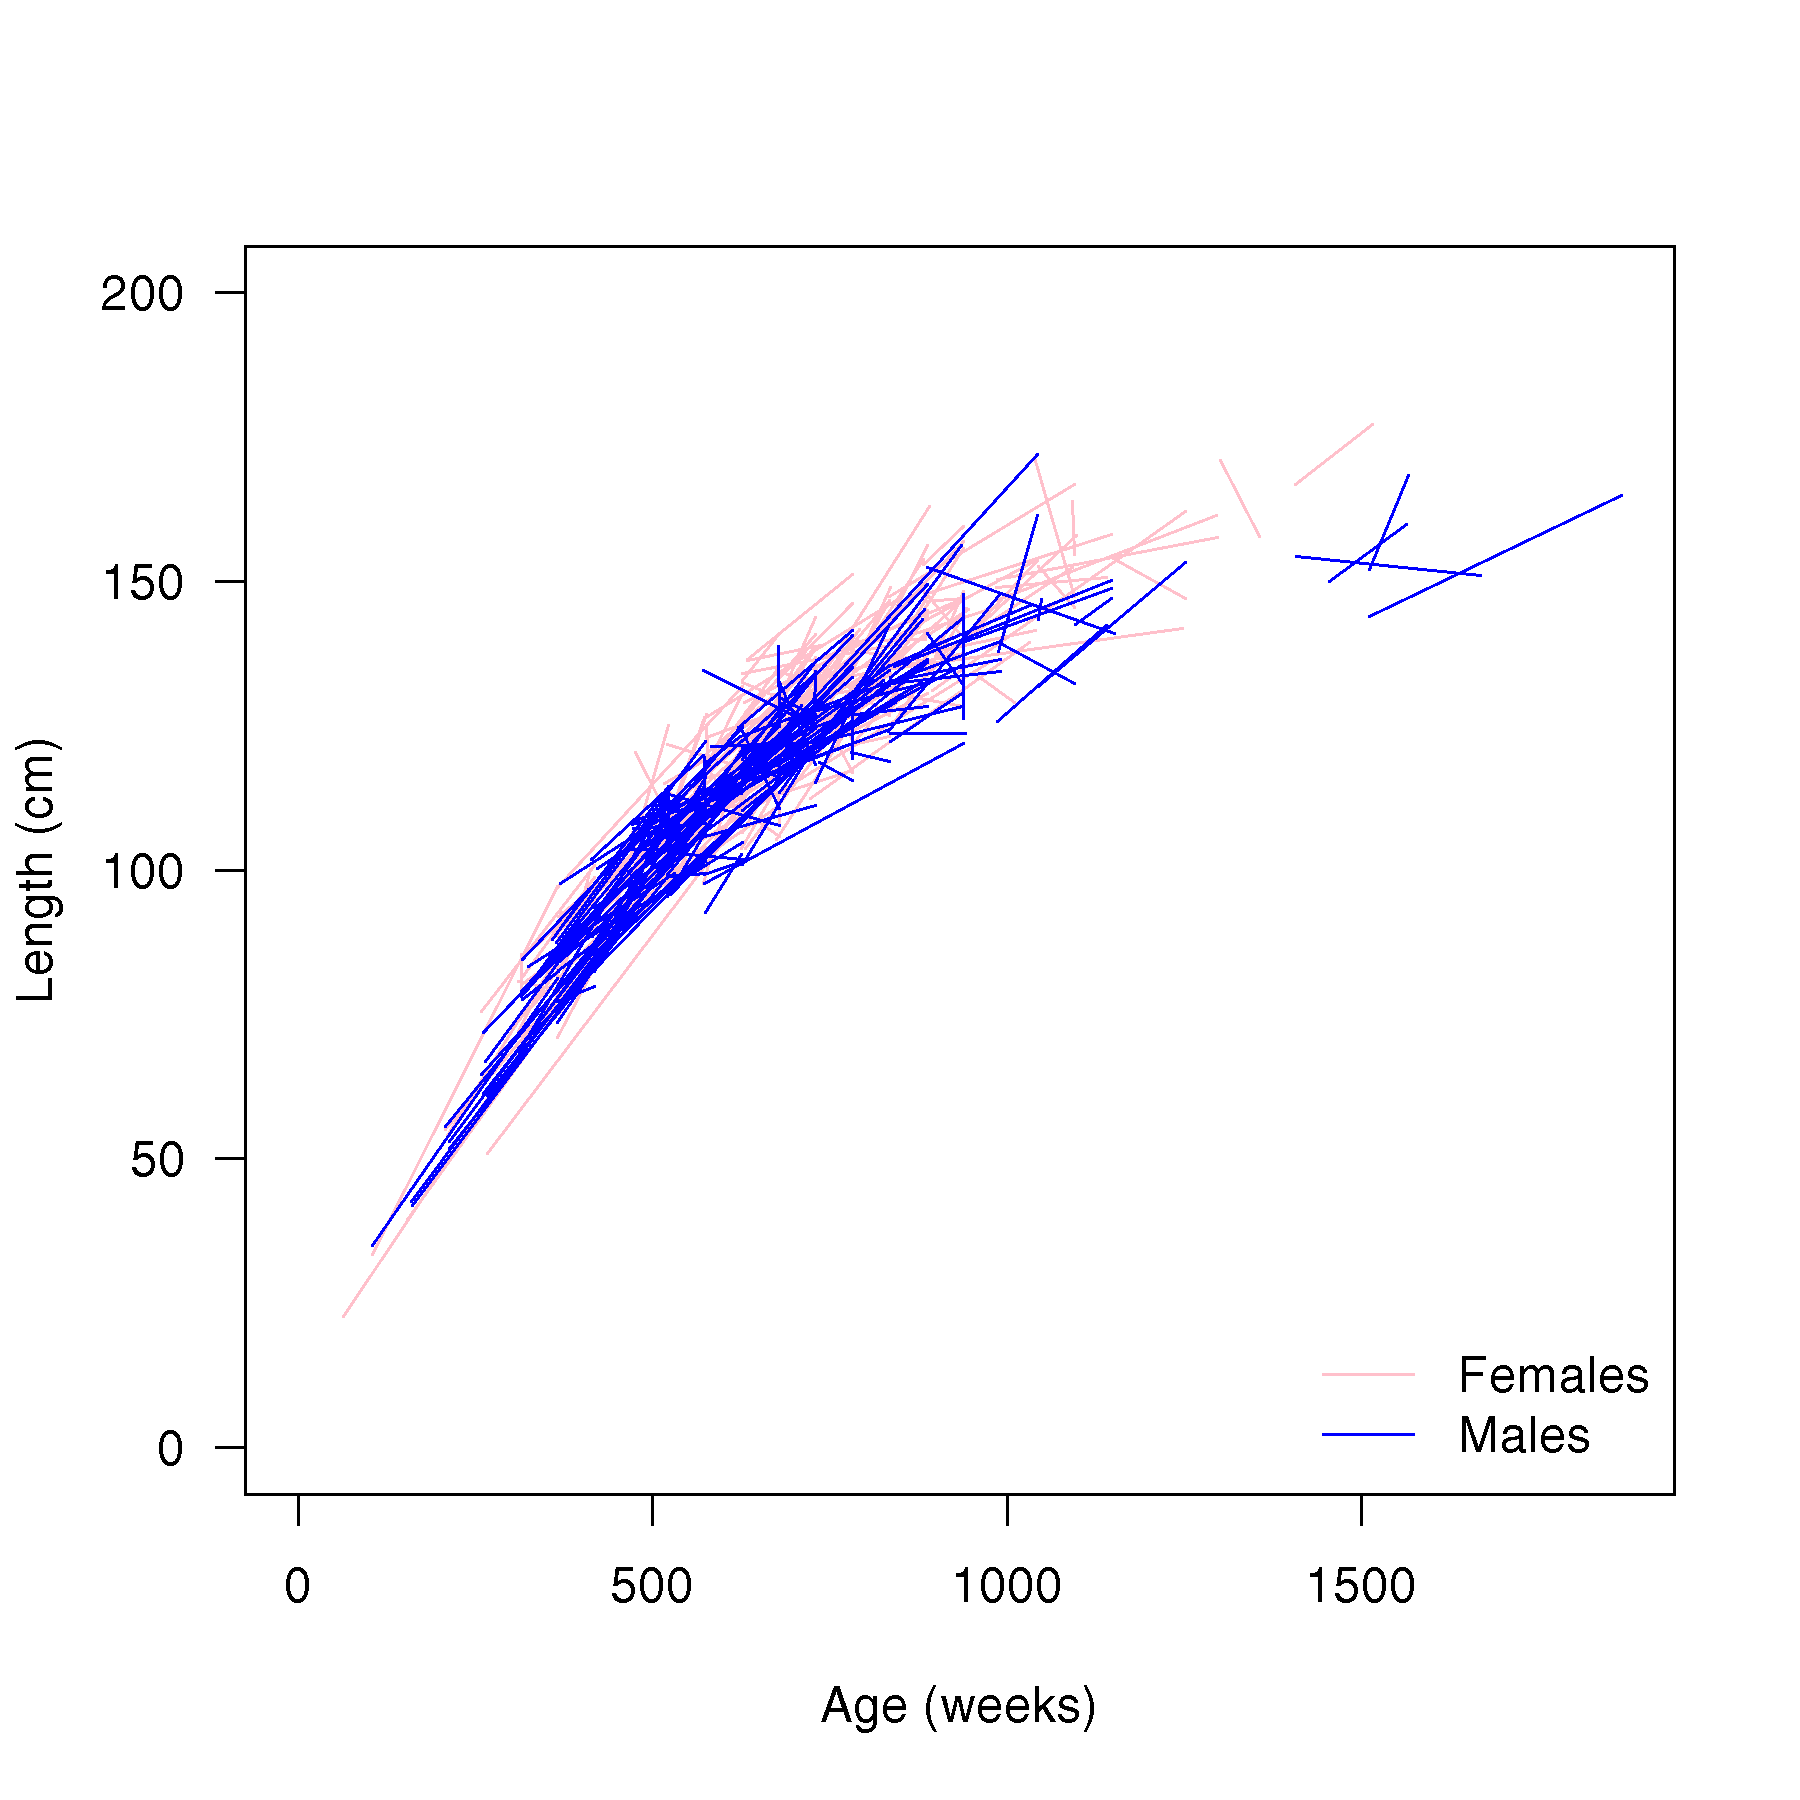
\includegraphics[width=0.49\linewidth]{../simulation/sims/growth-20.png}
  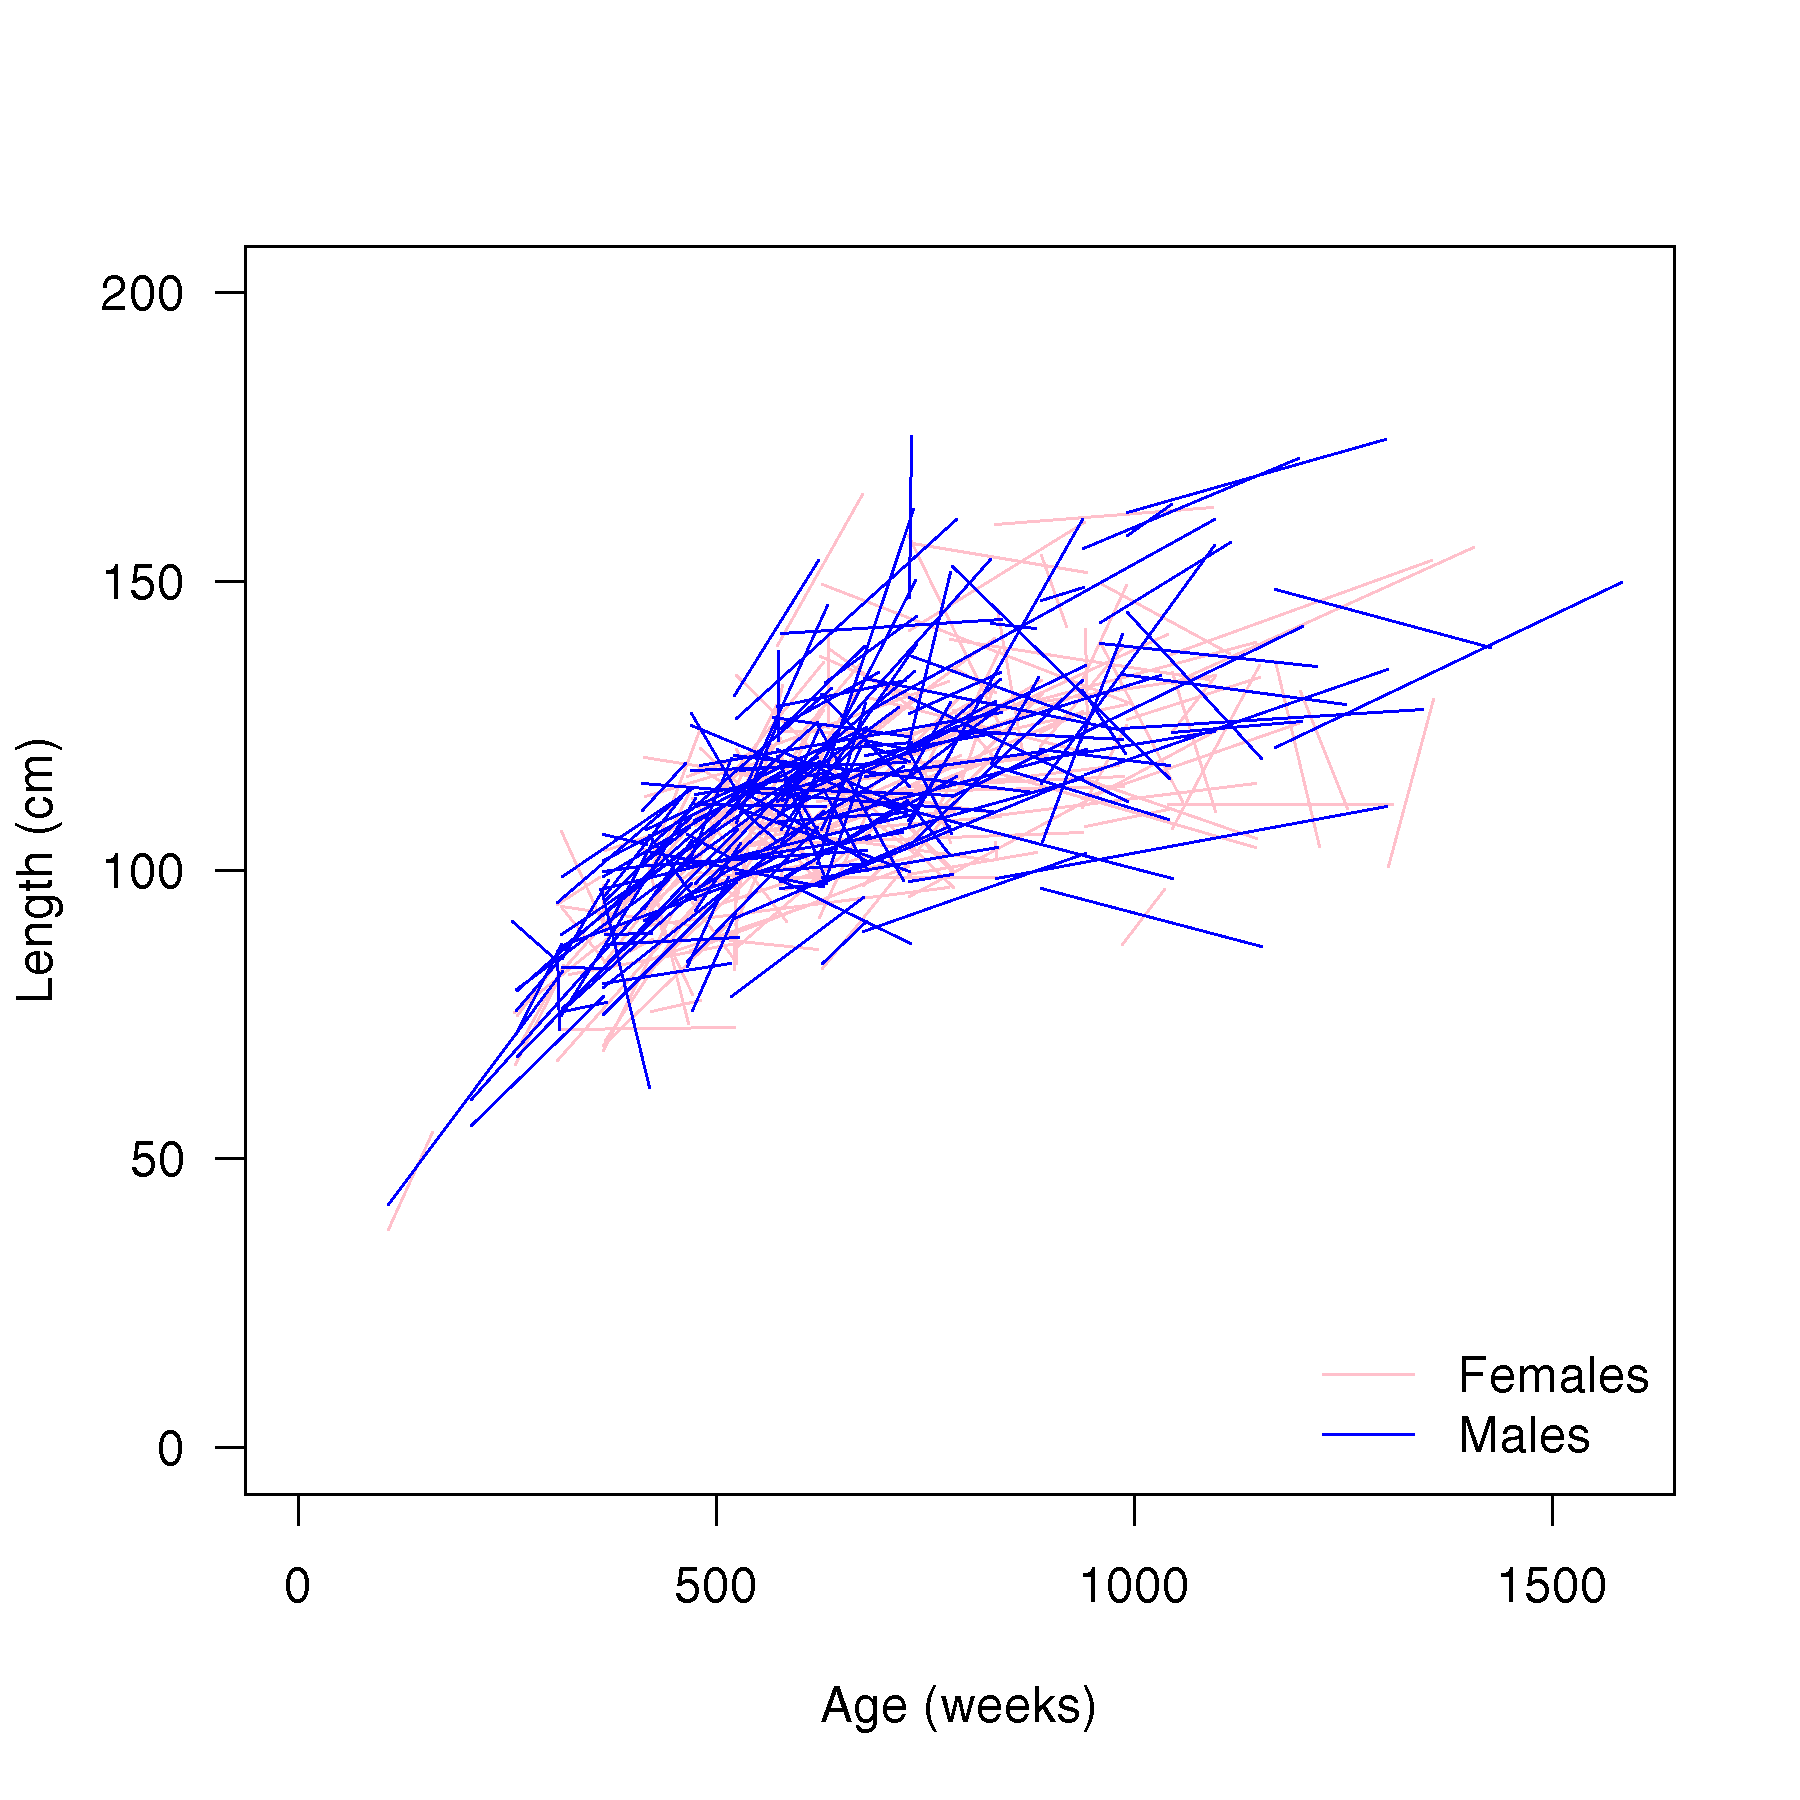
\includegraphics[width=0.49\linewidth]{../simulation/sims/growth-29.png}
  \begin{quote}
    \caption{Data sets for two models that were not pdH [top, simulations 1 and
      2], failed to converge [middle, simulations 6 and 45] and the only two
      datasets that were pdH [bottom, simulations 20 and 29].}
  \label{fig:1}
  \end{quote}
\end{figure}




\newpage\clearpage
%%%%%%%%%%%%%%%%%%%%%%%%%%%%%%%%%%%%%%%%%%%%%%%%%%%%%%%%%%%%%%%%%%%%%%%%%%%%%%%%%
\subsubsection{No random effects}
%%%%%%%%%%%%%%%%%%%%%%%%%%%%%%%%%%%%%%%%%%%%%%%%%%%%%%%%%%%%%%%%%%%%%%%%%%%%%%%%%
Here I tried turning of all random effects.
\begin{table}[!htbp]
  \begin{quote}
  \caption{\label{tab:} .} \small{
  \begin{center}
  \begin{tabular}{lrr}
  \hline
  Parameter      & Female & Male\\
  \hline
  $L_0$          & 0.0   & 6.9\\
  $\overline{b}$ & 0.003 & 0.003\\
  $\sigma_b$     & 0.0   & 0.0\\
  $\gamma$       & 0.4   & 0.4\\
  $\psi$         & 0.001 & 0.001\\
  $\sigma_o$     & 0.099 & 0.099\\
  $\sigma_z$     & 0.0   & 0.0\\
  $\sigma_y$     & 0.0   & 0.0\\
  \hline
  \end{tabular}
  \end{center}
  }
  \end{quote}
\end{table}

\begin{figure}[!htbp]
  \centering
  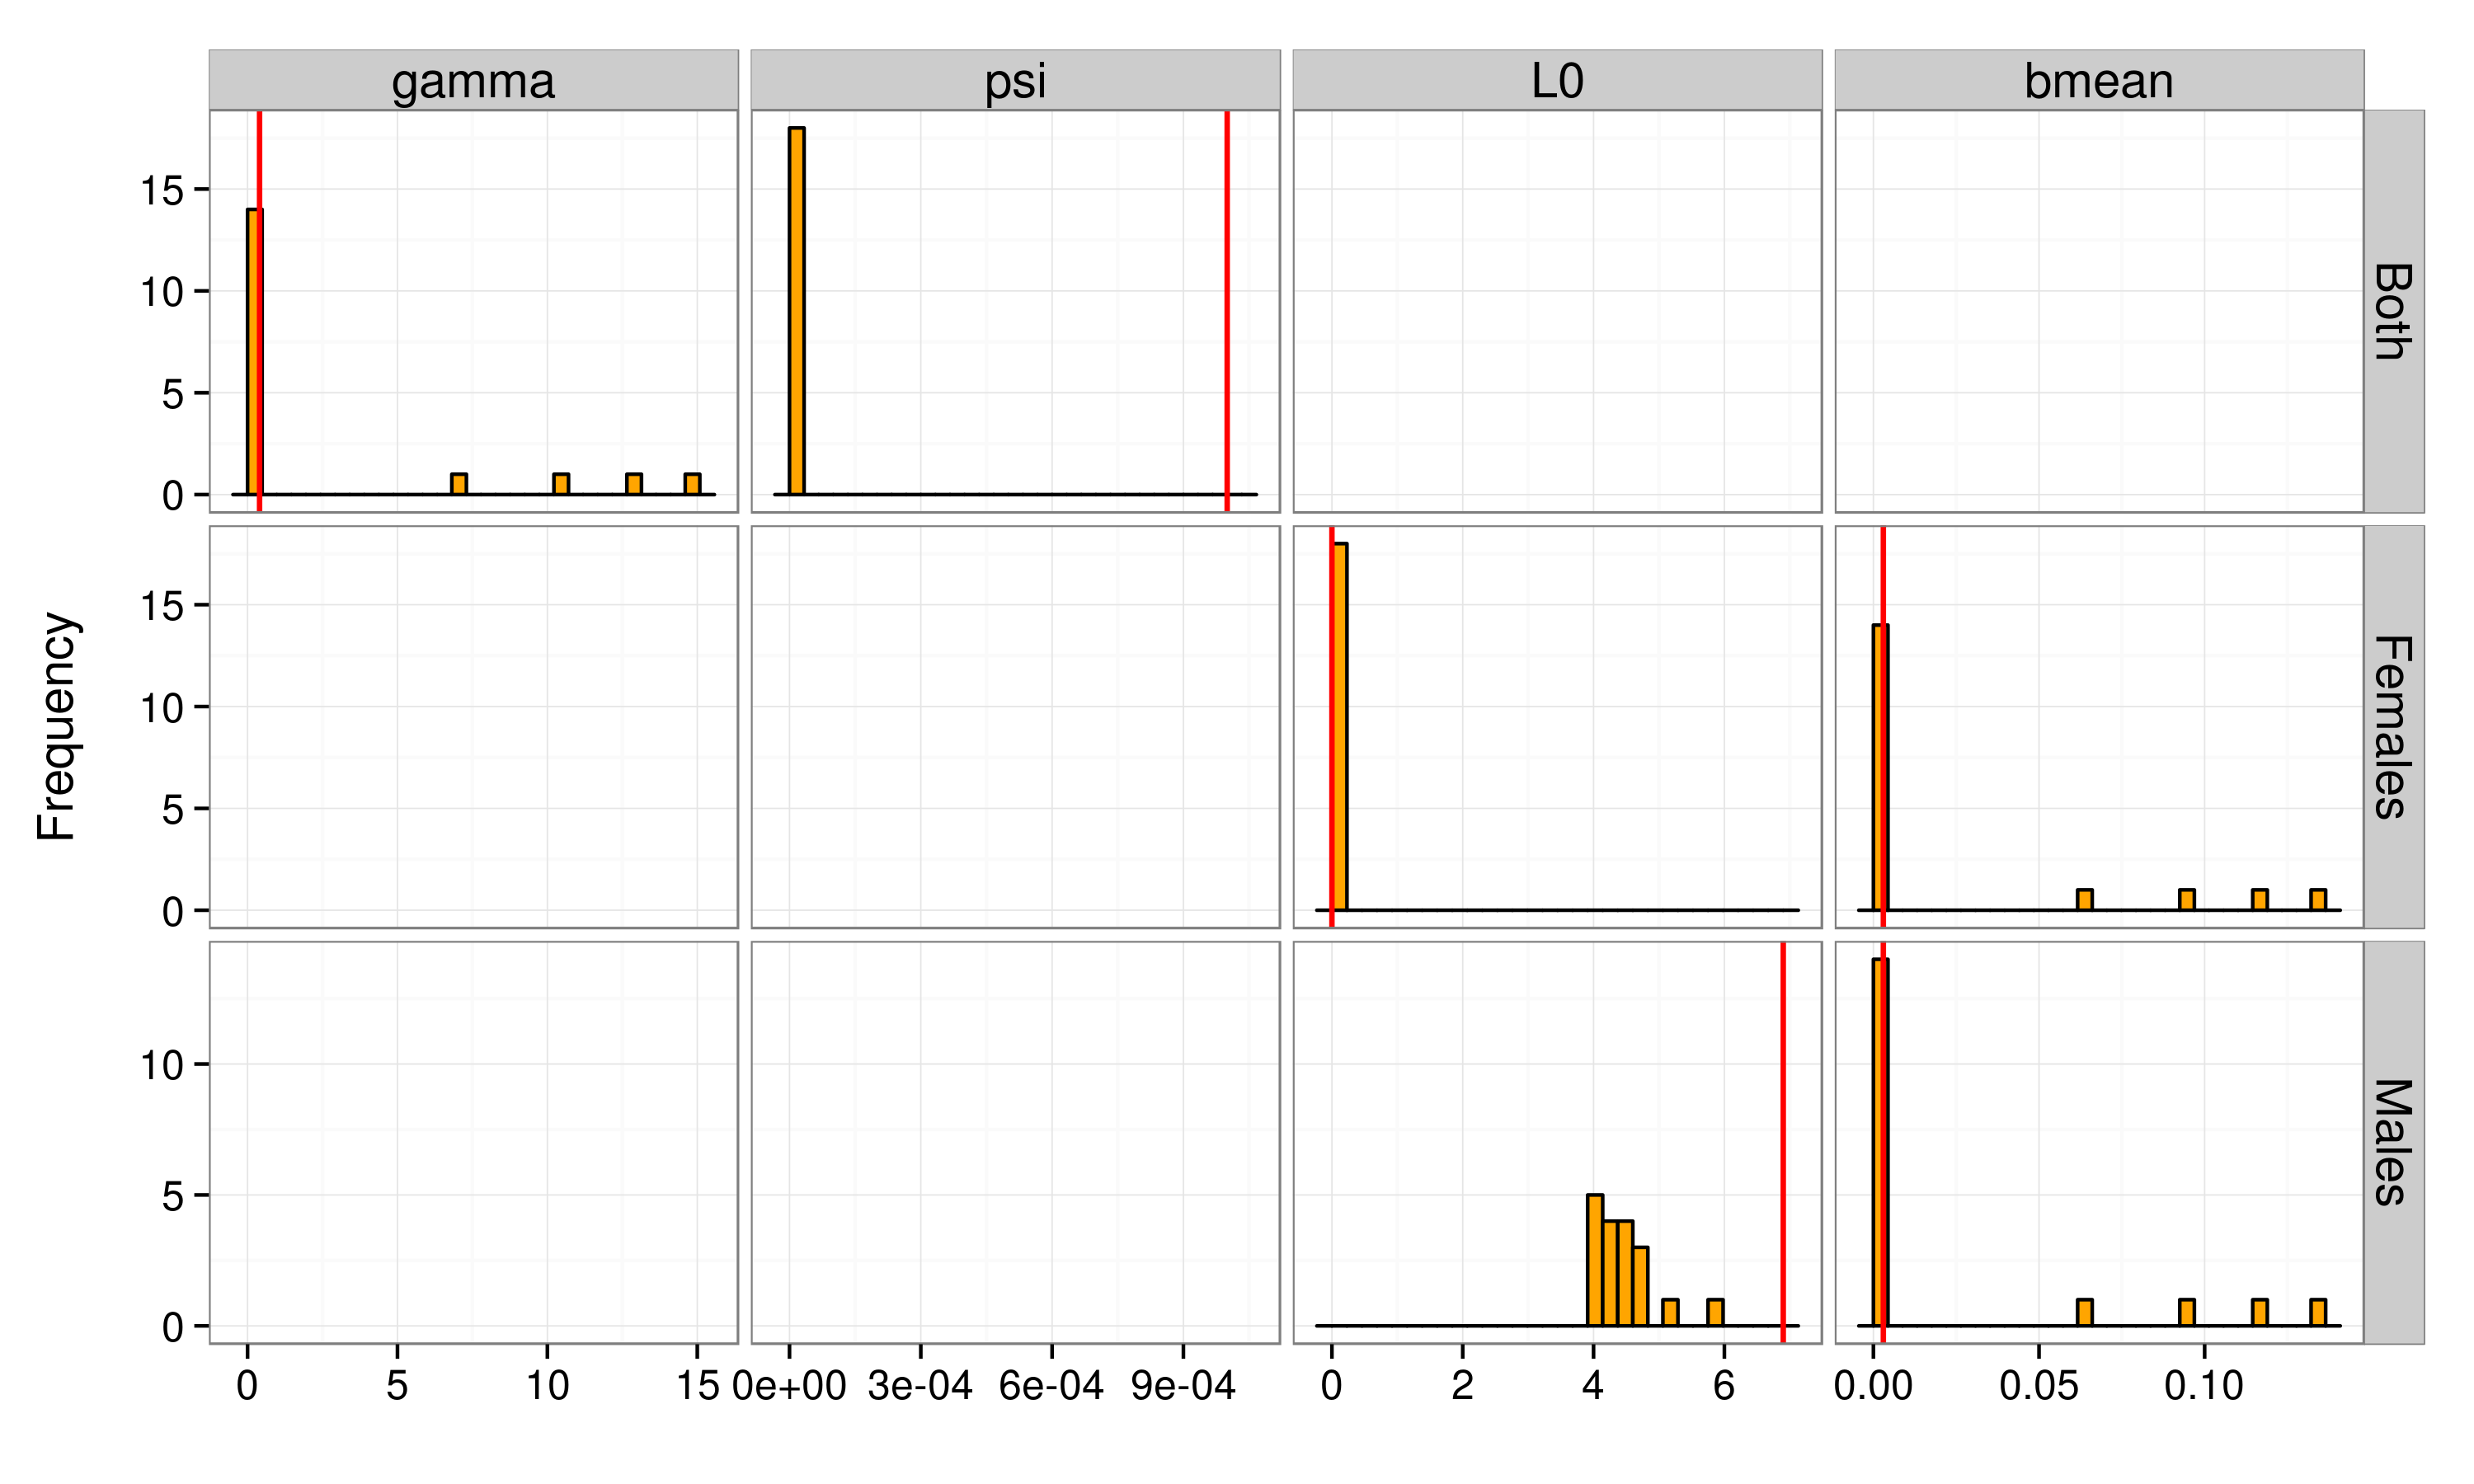
\includegraphics[width=\linewidth]{../simulation/sims/results/SimPars.png}
  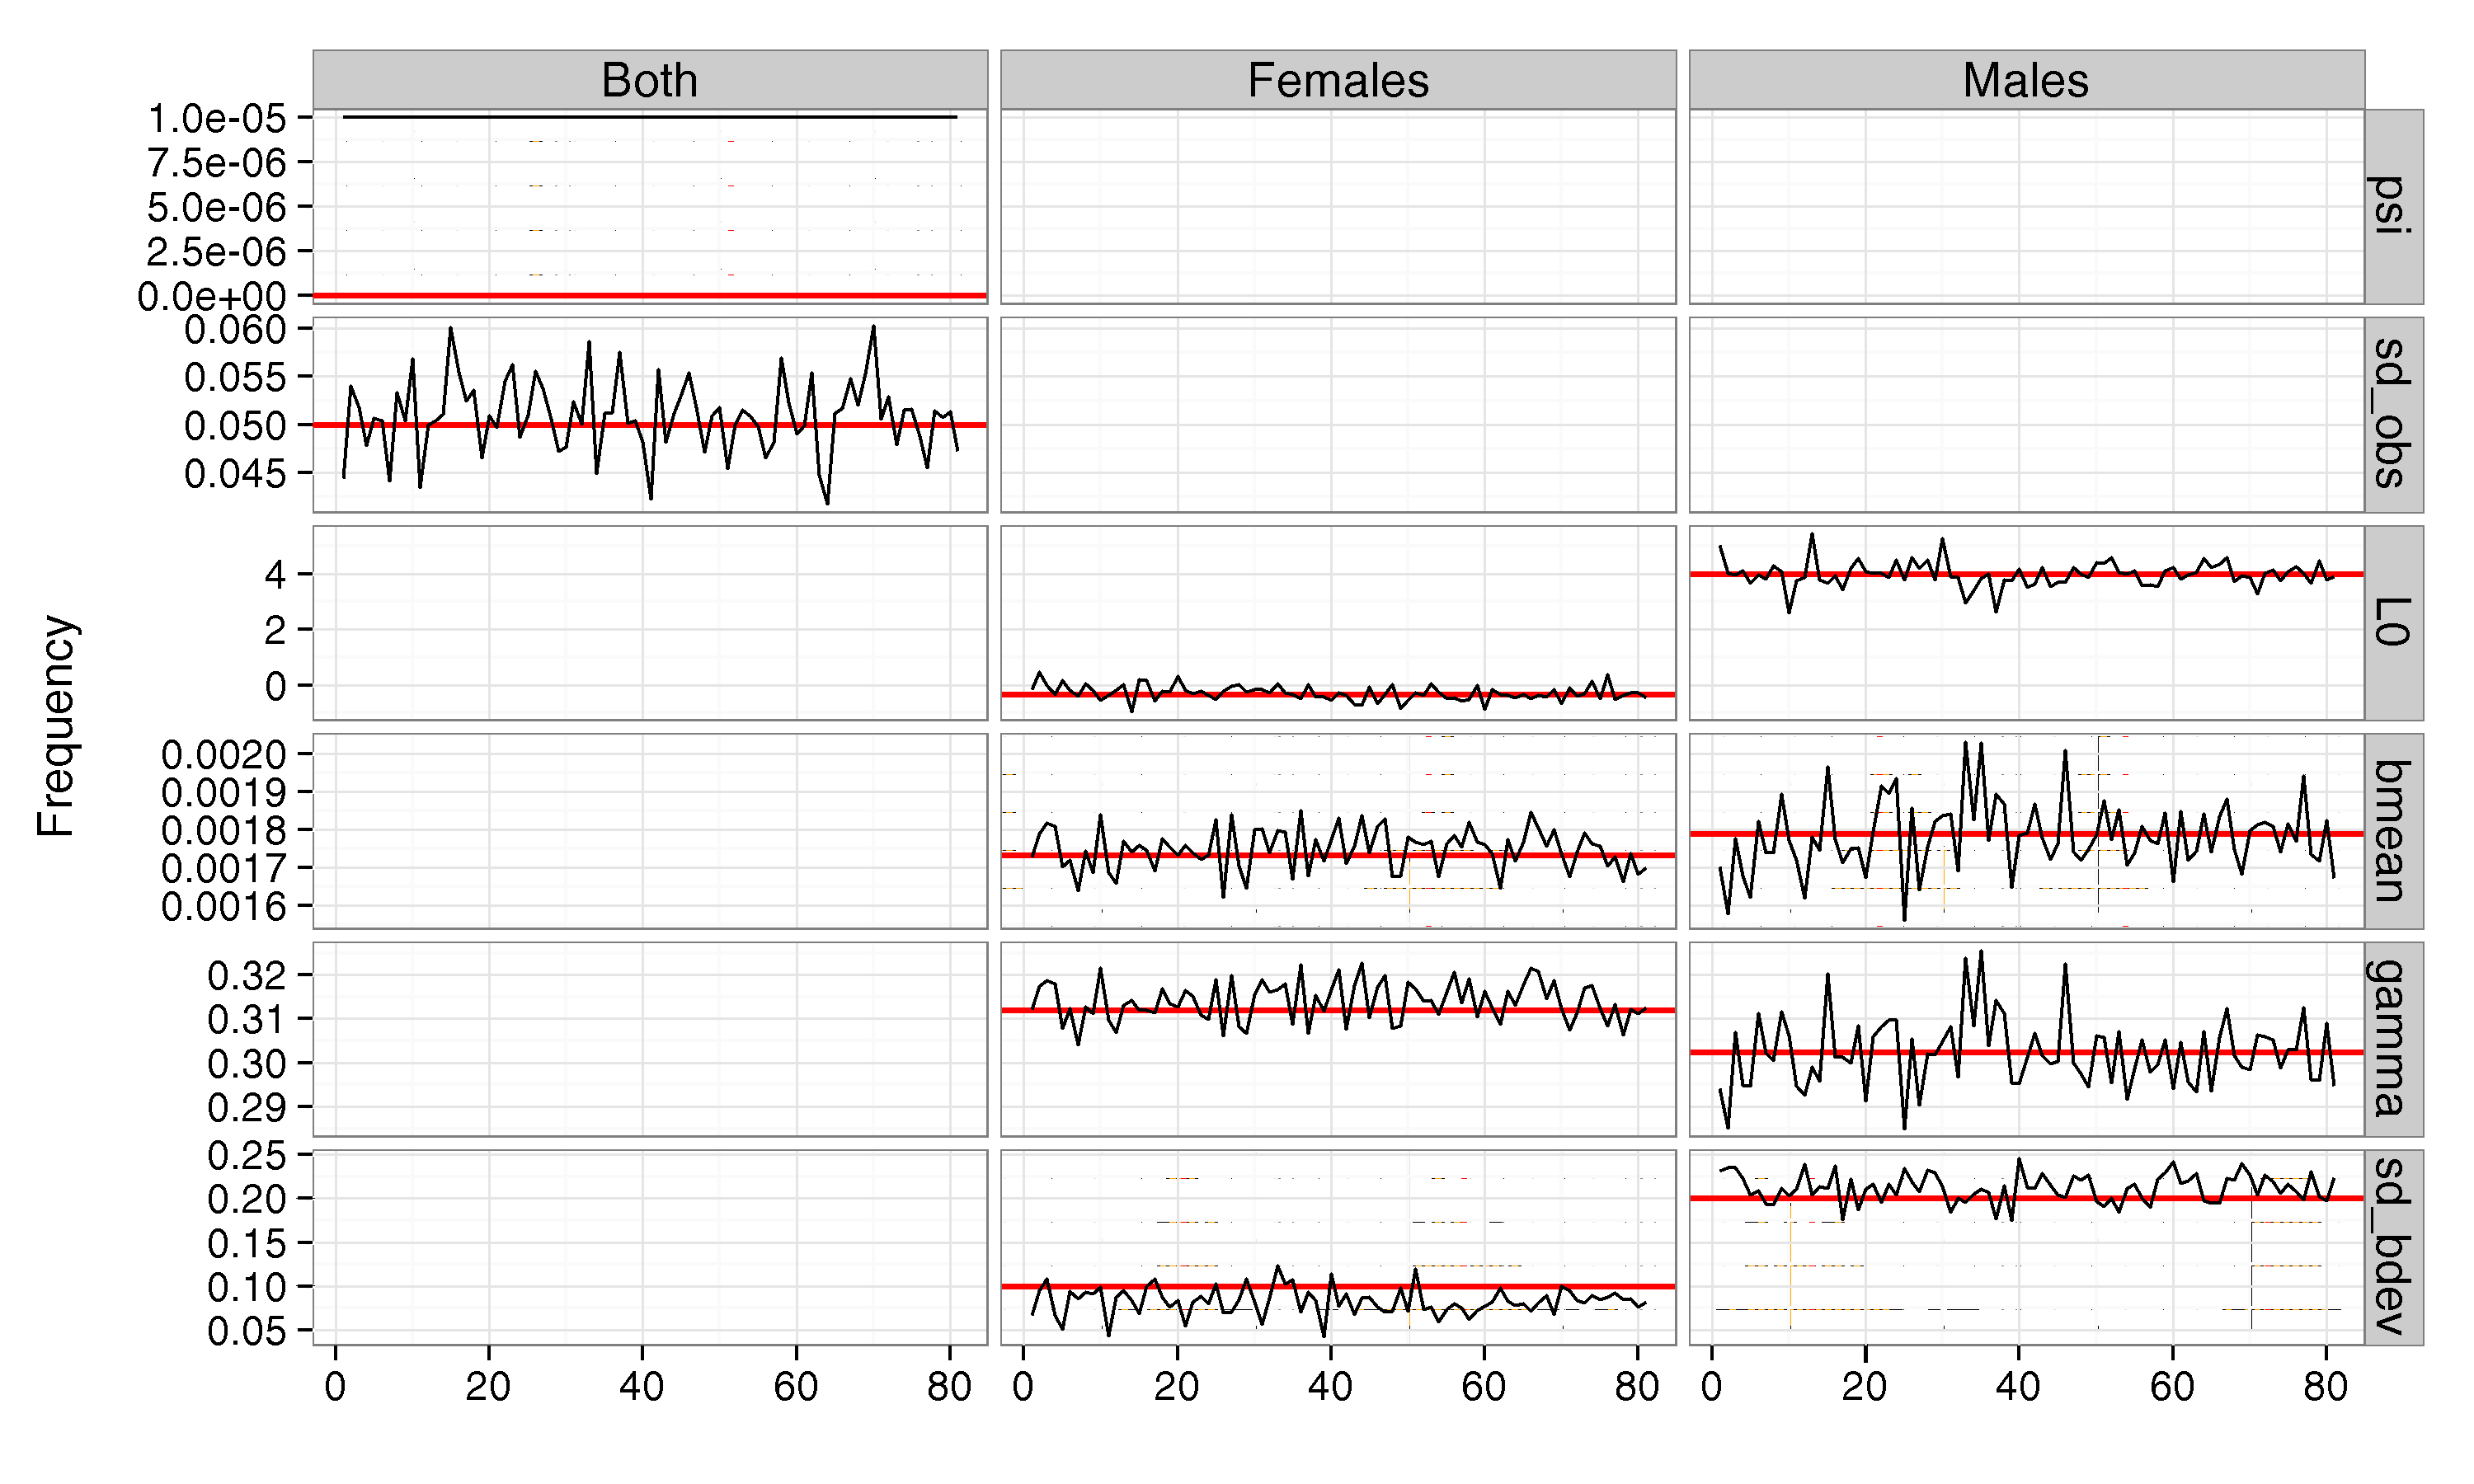
\includegraphics[width=\linewidth]{../simulation/sims/results/TracePars.png}
  \begin{quote}
    \caption{.}
  \label{fig:}
  \end{quote}
\end{figure}
